\label{chapt:portfolios}
The following sections give a holistic overview of various key groups
as the exist or existed circa 3276 CE (i.e. the UtCS period, see
~\ref{timeline:UtCS} and~\ref{exptimeline:UtCS}), combining factional, species, and aesthetic
information in a single place, from an omniscient viewpoint. These
portfolios are primarily designed to give insight and direction to
artists and other content creators. Much of the information here may
be duplicated elsewhere. There may be cases where the omniscient
viewpoint and in-game viewpoint disagree. Such disagreements are
likely intentional, reflecting misconceptions or ignorance on the
part of the extant groups. In cases where the disagreements seem more
ambiguous or unlikely in intent, please feel free to direct questions
as necessary.

\section{Cross-Portfolio Information}

\subsection{Faction Colors}

Faction colors exist for easier visual identification of factions and species. Factions from related species usually adapt similar colors with the exception of Humanity where the variety is too large to usefully allow using similar colors.

The faction color table (~\ref{fig:faction-colors}) below lists for each box

\begin{itemize}
\item Species and factions
\item Color name
\item RGB color value in real number [0.000 ... 1.000] range
\item RGB color value in natural number [0 ... 255] range
\item RGB color value in hexagonal number [\#00 ... \#FF] range
\end{itemize}

\begin{figure} \begin{center}
    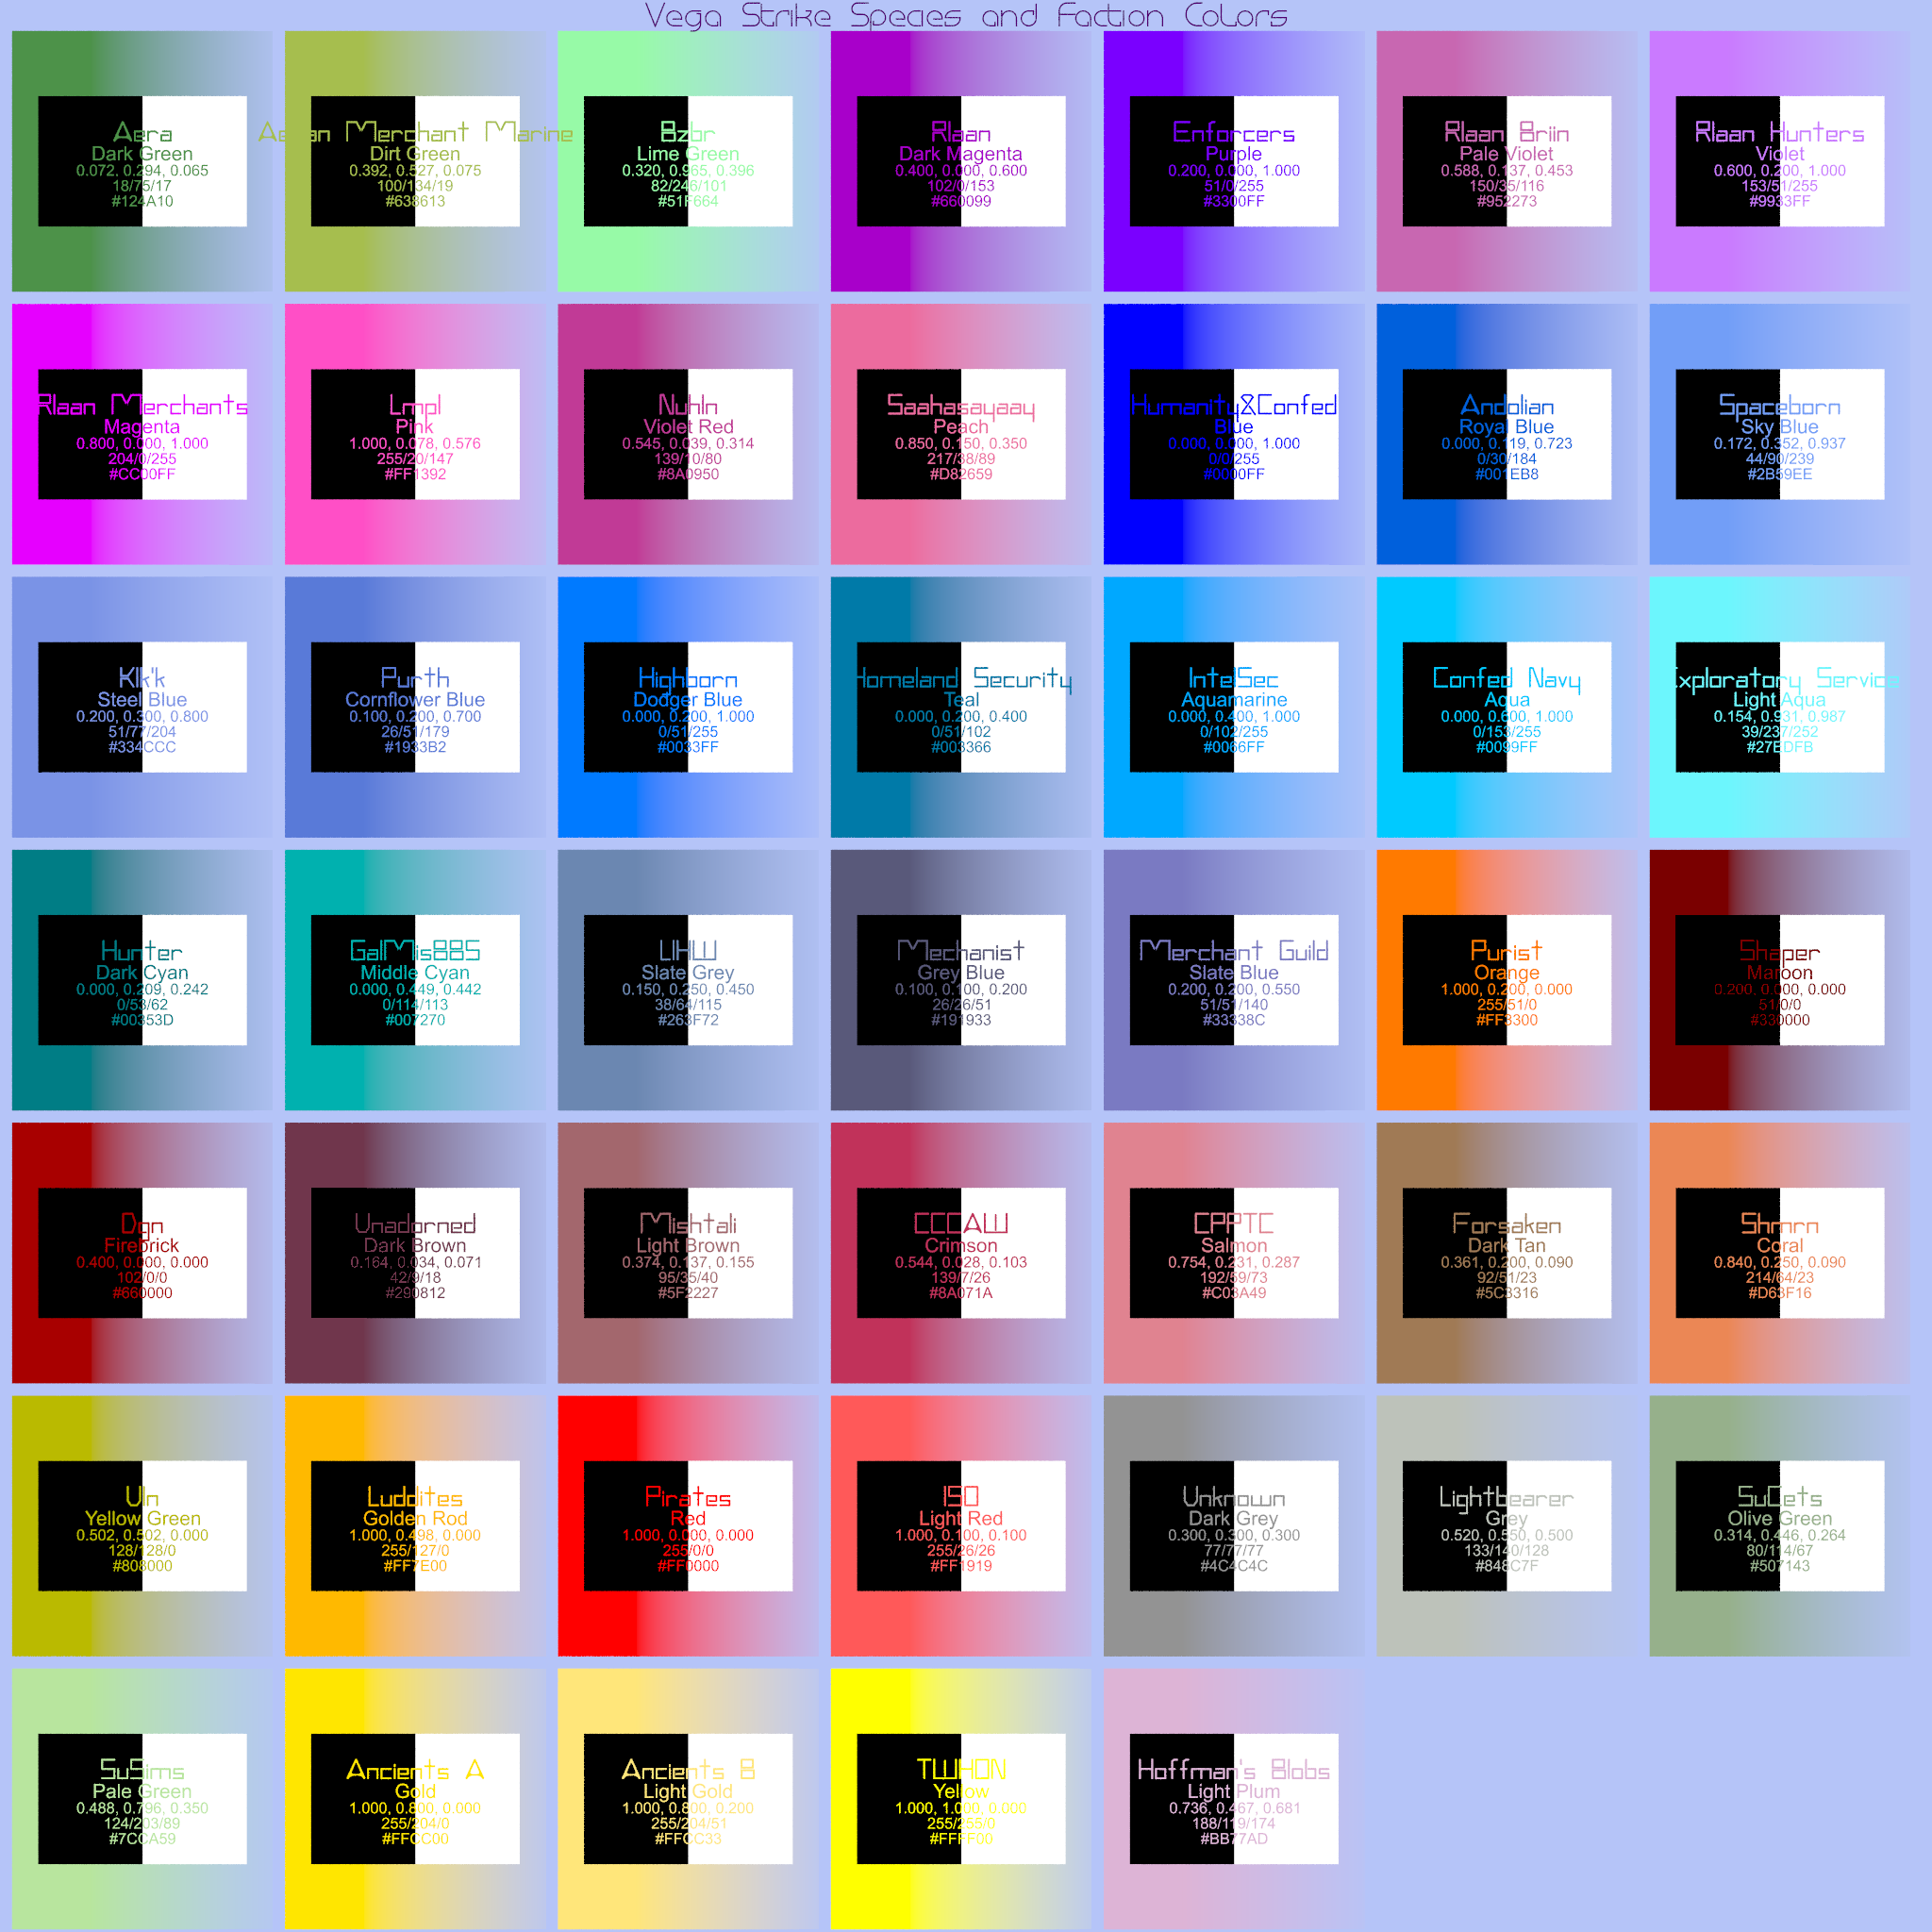
\includegraphics[width=1.0\textwidth]{../images/FactionColors_V1.png}
    \caption{Faction colors of the Vega Strike universe.}
    \label{fig:faction-colors}
\end{center} \end{figure}



\subsection{Vessel Overview}

\begin{itemize}
\item Engines

Retro thrusters, retro thrusters, retro thrusters, retro thrusters!
(to the tune of ``Developers, developers, developers!'')

If your craft is: A) not Rlaan manufactured and B) more than 5 meters
long it probably needs retro thrusters.

Now, the retro thrusters and maneuvering thrusters don't need to be
necessarily as pronounced as the rear engines (giving you some
artistic license in defining a visual front/back) but they NEED TO
HAVE VISUAL INDICATORS OF THEIR EXISTENCE. For some ships this is
mainly a texturing question. For larger vessels, this will necessarily
influence your model design.  

\item Radiators

One of the biggest problems in space is heat dissipation. VS
spacecraft have a lot of heat to get rid of, so they're going to need
radiators. While, as with retro and maneuvering engines, artistic
license is granted in how much of the ship's surface area is going to
be radiator dominated, the same need for visual indicators of
radiators exists. If you have fins, you should probably put a radiator
texture on them, because they're almost certainly not for aerodynamic
flight.  

\item Internals

VS ships aren't, in general, intended to be very dense. This is more
true for larger craft than strike craft. In general, the idea for VS
ships is that the surface-area to internals ratio should be pretty
high. The bigger ships in VS can be seen as big shells of armor and
radiators around many, smaller, internal components. Moreover, a lot
of the internal components would actually be plumbing, of the coolant
(I always had a soft spot for gallium alloys, but no decisions are
finalized on what exactly the coolant is) circulating variety, running
between the reactors/engines (the engines being fusion reactors
themselves) and other heat-generating components (e.g. weapons). The
rest of the space being taken up by insulation (vacuum is pretty good)
and physical shielding to keep the crewed and other sensitive parts of
vessel safe from the engines/reactors, and other hazardous portions of
the ship.  

\item Atmospheric flight

Most spaceships in the VS universe, even if capable of accelerating to
escape velocity, are not designed for atmospheric flight. Some are. If
its role description mentions ``Aerospace'' or ``lander'', ``puddle
jumper'', ``dropship'', ``ground support'', or ``orbital'' then it's a good
bet it has an atmosphere-friendly design. If not - build a spaceship,
not an airplane.

That said, some smaller craft that are not atmosphere-friendly will
still be atmosphere capable. The more developed the infrastructure of
the group using/designing the ship, the more likely they don't intend
for it to ever see atmospheric use on an inhabited planet - this is
what docking stations, space-elevators, orbital shuttles, and other
infrastructure exists for. In fact, (once we get planetary structures
squared away a bit better), the really industrialized planets will
probably start firing on you if you attempt to land in anything larger
than a pinnace/dispatch craft, and even then only with appropriate
permission. On the flip side, if it's a Forsaken ship, or a Luddite
craft, then it probably spends a lot more time visiting places without
well-developed orbital infrastructure and may need to land on
occasion. Also take into account the age of the design you're
considering. Much of the VS universe as of 3276 is post-frontier, but
a lot of places don't have to think back too far to remember when they
weren't. Use your better judgment.

If the ship is very large, even if it is atmosphere-capable, it is
almost certainly {\em not atmosphere friendly}, unless perhaps it's
something very esoteric (atmosphere skimmer for terraforming project
or some such). In general, if the ship is very large, it's best to
assume it's not even atmosphere capable unless there's a very good
reason for it. Large vessels will make use of shuttles and dispatch
craft to take care of business on the ground.

\end{itemize}


\section{Portfolio: The Aerans}
Ships overview for all groups (Work In Progress): \href{http://vegastrike.sourceforge.net/wiki/Artstyle\_guide:Overview\_Guide}{Ship Overview} \\
Art-style Guide (Work In Progress): \href{http://vegastrike.sourceforge.net/wiki/Artstyle\_guide:Aeran}{Artstyle Guide} \\
Species overview: \href{http://vegastrike.sourceforge.net/wiki/Species:Aera}{Species:Aera} \\
Faction overview: \href{http://vegastrike.sourceforge.net/wiki/Faction:Aera}{Faction:Aeran Ascendancy}

\subsection{Origin}
\begin{itemize}
\item Gravity: ~1.3x Earth-normal

\item Atmosphere: Nitrogen-Oxygen (24\% O2), with minor nobles (neon, argon), carbon dioxide, and water vapor

\item Primary liquid bodies: water, ~80\% surface cover, continents small, large islands frequent

\item Average temperature of homeworld (pre-industrialization): ~300K

\item Sun: Orange

\item Primary challenges (pre-industrialization): Extremely competitive and invasive ecology.
\end{itemize}

 An intelligent centauroid species which developed on a misbegotten
hell of a jungle world, the Aera are oxygen-nitrogen breathers, with a
strong internal skeleton, smooth ashen-gray leathery skin, a decided
lack of psychiatric assistance for their obviously repressed
dissatisfaction with natural ecology and, at least according to the
Cult of the Devourer on Mishtal Seven, a flavor remarkably similar to
that of a human with a high protein diet, but only if both have been
served with a nice Chianti.

Unfortunately for the Aera, their region of the jump network offers no
known paths towards significant further expansion. To expand they must
go coreward, passing through Human or Rlaan controlled
systems. Requests to do so have been denied by both the relevant
parties of both species. Opting for another method, the Aera tried to
sneak a colony convoy through Rlaan space, but a lack of comprehension
of the Rlaan mentality regarding civilian casualties caused this ploy
to be not only a failure but a disaster, provoking the Rlaan into a
military response.

\subsubsection{Habitat}
The Aera homeworld was, prior to changes imposed by the technological
advancement of the Aera, a nearly seasonless planet with an
oxygen-nitrogen-neon atmosphere, on whose surface were a single large
landmass and many large and small islands. The mainland was nearly
entirely covered with jungles and marsh-groves, with only small belts
of more sparsely overgrown land on the northern and southern reaches
of the continent. The rich jungle land was home to all sort and manner
of parasites, predators, diseases, and competitors for food. It was in
this vast, dark jungle that the Aera arose into sentience, tool use,
and civilization.

\subsection{Physical}
\begin{itemize}
\item Dimensions: 2-3 meters in length from the head to the end of the balancing tail. 1 - 1.25 meters high at each of the the four leg-shoulders.

\item Mass: 200-250 Kg

\item Skeletal system: Multi-vertebrate(4) with interleaved rib arrangement, bilateral symmetry

\item Major divisions: Tail, midsection (hind-limbs to mid-limbs), fore-section (mid-limbs to arm-shoulders), neck, head

\item Senses: Audio, visual, chemosense (all in head). Tactile (skin, strongest at hands, rear-feet, tail)

\item Visual acuity: Aera cannot see in the dark, but do have excellent low light vision. Long distance focus is inferior to that of humans, but motion sensing and clarity of short and medium ranges is superior to human norms. 

\item Chemosense: Aerans have both external (lower face) and internal (mouth) chemosense organs. Aerans are mouth breathers, and do not have nasal passages. External chemosense organs are used primarily to assist in lending directional information to scents picked up by the internal chemosense organs. 

\item Locomotion: The ancestors of the Aera ambled about amid the lowest layers of a continent-spanning, towering jungle. The Aera prefer to scamper as often as walk, and move on their mid and hind-limbs, their fore-section parallel with the midsection, arms tucked in, and tail extended for balance.

\item Manipulators: Two hands, each with a 2+1 finger/thumb arrangement

\item Textural appearance: Leathery skin, thick over most parts of the body. Ashen gray, with darker gray striations and amorphous, blotchy, yellowish patches in a pattern unique to each individual Aera
\end{itemize}

The Aera are a centauroid species measuring 2-3 meters in length from
the head to the end of the balancing tail, and 1 - 1.25 meters high at
the four leg- shoulders. The four stocky, sturdy running/gripping
limbs provide support, and the front two limbs end in three-digit
hands, with two fingers and an opposable thumb. When active, the upper
body bends up from the rest of the body just past the middle limbs at
about a sixty-degree angle, with the forelimbs sprouting from about
two thirds of the way up the upper body, and with the head bending
back down so as to be parallel with the main trunk and the
ground. Aera tend towards slim, muscular builds, and are usually both
quick and agile. They have two genders, each of which is similar in
appearance. Among the space faring races, the Aera have one of the
shorter natural lifespans. Prior to the advent of advanced life
extension technologies, it was as rare for an Aera to reach 60 years
of age as it was for a twentieth century human to reach 100.

The physical appearance of the Aera reflects upon their origins. The
Aera have a smooth, leathery skin not dissimilar in appearance to the
bark of a birch tree, with occasional yellowish patches reminiscent of
lichens. The hinged portion of the mouth is, in contrast to that of
Terran species, the upper portion. The mobile portion of the mouth is
also notable in that it does not consist of a bony arch, and is
actually a solid bony plate. Inside this mouth are two rows of teeth,
the second moving forward to replace the first as they naturally fall
out, and a new second row is grown. The front teeth are razor sharp
and are obviously for tearing flesh, and the next sets of teeth are
likewise designed for the chewing of meat, but the rearmost few teeth
have grinding surfaces, allowing the consumption of nuts, seeds, and
other such vegetable matter. The corners of the mouth are usually
open, and provide the normal breathing route. When exerting itself, an
Aera will pull back its lips, increasing the size of the airway. The
wide, narrow eyes are almost universally a milky green, with wide,
narrow pupils, and are largish in size relative to the head. The eyes
are above the terminating point of the downward slant of the lip-line,
but below the bony jaw plate. Just below the mouth, on each side of
the head, is a row of small pits that are used for
chemoreception. Beneath each eye is a kidney-shaped patch of lighter
skin that marks the location of a tympanum. On the underside of the
Aera head is a pair of organs, each capable of producing variable
amplitude, low frequency vibrations, which the Aera use to
communicate.

NOTE: depiction of head in Figure~\ref{fig:Aera-body} is non-canonical, picture otherwise highly informative:   Basic body plan is captured reasonably by
\href{http://vegastrike.svn.sourceforge.net/viewvc/vegastrike/trunk/document\%20generation/images/Aera.png?view=markup}{Aeran Body Plan}
but the head is entirely wrong, and the coloration is a bit off (so
ignore the head and the coloring should be closer to gray than white).

\subsection{Mental}

The Aeran thought processes mostly operate at speeds comparable to
that of humans, but with some notable distinctions in process,
efficiency and valuation of concerns. On average, Aerans possess
demonstrably superior quantitative reasoning skills compared to human
norms. While not completing most subtasks at remarkably faster speeds,
Aerans are much less likely to make mistakes or become lost or
distracted. Compared to humans, Aerans are at once chronically
hyper-alert, but capable of obsessive levels of focused concentration
on the task at hand. Aerans do not degrade in mental capacity as
readily due to exhaustion. In general, the entire Aeran body will
operate at near-full capacity through extended non-rest and stress
periods, collapsing in a step-function, rather than gradual
manner. Indeed, the Aeran existence is one of nearly constant stress,
as they work themselves to death in lives far shorter than that of
Humans, Klk'k, etc. Humans would consider all Aerans to have a
thoroughly paranoid mindset. Aerans feel their concerns are entirely
rational, as, historically, most things {\emph have} been out to get
them. Aerans have extremely strong hierarchical loyalty arrangements,
and, although possessed of individuated desires, excel at subverting
them to the demands of the hierarchy. Through countless wars of
successive integration and the institutions supporting the Aeran
cultural and political hierarchy, the loyalty structure of the Aerans
has enabled them to map their natural pack/clan bond affinities onto a
profound species-wide affiliation. The primary goal of Aeran society
is what it has always been: group survival above all else. All that
has changed is the parameters and implementation details. While the
Aera are not innately belligerent, they are innately non-trusting and
tend towards presumptions of negative intentions on the part of the
other species they have had relations with. Moreover, when the Aera
feel threatened, it is easy for them to justify arbitrarily extreme
measures if they believe said measures will at all increase the odds
of their long-term survival. As such, the policies pursued have often
been seen as startlingly aggressive by the other parties involved.

\subsection{Technological}
\begin{itemize}
\item Tech: 

Aerans excel at most applied mathematics and the physical sciences,
but lag noticeably in biological sciences. Aerans clear-cut their own
homeworld, driving back their ancestral jungles to make room for their
industrially-oriented civilization, and prefer living entirely apart
from the ecosystems of the worlds they colonize whenever
possible. Aeneth-forming relies heavily on cleansing the host-planet
of its native ecologies before introducing Aeran ones. Aeran
colonization is a very infrastructure-intensive task compared to the
techniques deployed by humans and even more so in comparison to the
Rlaan. Aeran society in general is very resource intensive. While the
Aeran rate of population increase and technological progress is very
rapid, they left their homeworld much later than the other
interstellar powers, and the further reaches of their empire are much
less developed. While the planet is being rendered amenable, the
Aerans will tend to focus on developing orbital infrastructure even
while little-to-nothing exists on the ground, and will do so to a
greater degree than other groups. The Aera shun fully autonomous AIs,
as they view them as more likely competitors than allies. They view
biological AI constructs in much the same light. AI research is
therefore somewhat stunted in Aeran society, and certain tasks are
thus much more labor-intensive. Aeran research in weapons technology
is excellent, and frequently somewhat superior to that of the other
factions. However, a bias toward excellence has skewed the
quantity-quality trade-off somewhat toward quality over
quantity. While the Aera will not forsake economic or practical
efficiency wholesale, they are innately comfortable with the notion of
problems being solved by the introduction of superior technologies and
engineering. While Aeran technological and engineering progress is
rapid, they are making up for lost time relative to the other species,
and their advancement is uneven.

\item Weapons:

Aerans have a notable preference for shield-piercing weaponry and tend
to ignore options without significant shield-piercing effects. The
Aerans wish to make every shot count, and are thus more limited in
their potential array of death-dealing options. Most smaller Aeran
weapons are ammunition based, utilizing complex warhead designs that
emit a brief, intense pulse of radiation upon contact with an enemy
craft's shields. The preference for shield-piercing weaponry extends
to Aeran capital vessels and missile designs. Aeran craft tend to
prefer using larger numbers of smaller missiles over smaller numbers
of larger missiles.

\item Tactics:
\begin{itemize}
\item    Small groups: smaller Aeran craft, while purposed, are capable of generalist missions and are often tasked with recon and commerce raiding 
\item    Large groups/Fleets: Aerans prefer large engagements to skirmishes, as they tend to be more direct in attempting to achieve their goals. 
\end{itemize}

The primary use for small craft in Aeran fleets is as a screen for
larger capital vessels. Aeran interceptor craft are defensively
oriented. In contrast with many other groups, the vast majority of the
superiority fighters will also remain behind to guard the
fleet. Corvette class vessels are the primary implements of Aeran
assaults on other fleets. The Aerans do not rely on what would
generally be considered bomber class vessels, and instead utilize a
mix of assault corvettes, F/A light craft, and escort corvettes, the
latter two acting as the primary escorts for the torpedo-rich assault
corvettes. Capital vessels engage at maximum distance, and attempt to
remain at distance from enemy fleets until the enemy's organization
has been broken, or the fleet's missile supplies have been
exhausted. Larger Aeran capital ships, even in their non-missile
load-out, generally prefer a role more artillery than cruiser in
nature. While Aeran destroyers are capable generalists, the majority
of their armament is tailored to engaging assault vessels and other
larger, less maneuverable sub-capitals. However, Aeran destroyers do
tend to have very solid forward acceleration and the ability to orient
all primary turrets in a forward direction for chase maneuvers. Aeran
craft built specifically to counter threats in the Rlaan-Aeran
conflict have a disproportionate number of weapons designed to deliver
maximum damage over short time periods at short distance. Larger Aeran
capital vessels are on the larger side, and significant economic
investments for the Aera, even relative to most other major
factions. The Aera will readily sacrifice smaller vessels to allow
their larger assets to escape a losing engagement. While the Aera
operate what is arguably the largest carrier currently in use (the
Agesipolis), it is used more as a mobile base, moving in to hostile
systems only after initial combat operations have subsided. The Aerans
instead rely on jump-capable small craft, even for purely defensive
scenarios, and a larger number of much smaller tender craft
(currently, the Dorissus class) to repair, refuel, and rearm
them. This is in keeping with the much larger role of sub-capital
(non-fighter) craft in the Aeran fleets, and their ability for
self-management relative to fighter-craft.

\item Installations:

Almost all Aeran installations are armed, and any sizable one armed
heavily. The Aera are very reliant on their orbital infrastructure,
and will go to great lengths to defend it.

\end{itemize}

\subsection{Culture}
Aera culture is highly organized and decidedly hierarchical, but in
the form of a meritocracy rather than an aristocracy. While what has
constituted merit has morphed over the millennia since the first Aera
tribes selected work crews to cut back the encroachments of the jungle
upon their early settlements, given the relative position of the
pre-technological Aera in their local food chain, there has long been
a favoring of cleverness and determination over raw strength. The
current social and vocational position of any Aera is immediately
indicated by the color and pattern of an individual's coverall. The
Aera are ruled by a subset of the highest caste, with membership in
the oligarchy changing whenever either an individual steps down, or a
third of the other members call for a member's replacement. New
members must be confirmed by two thirds of the current oligarchy. It
is much more common for members to voluntarily remove themselves from
power, believing themselves more useful elsewhere in society, than to
be cast out. An average stay in the oligarchy lasts a few Aera years.

The long struggle of the Aera against the erosion of their society at
the hands of the natural world has instilled in them a deep respect
for that which has enabled them to conquer their environment:
technology. Not only is the advancement of technology greeted without
fear, the social position of the artificer and the engineer is one
more greatly elevated than that seen in any pre-Diaspora human
society. What is feared is the unmastered and uncontrolled. Even after
the last war between Aera and Aera was fought, bringing the last of
the major islands under the control of the mainland, the Aera only
slightly relaxed their military investment. Perhaps in large part due
to their short lifespan, and the consequential rapid dying off of
adherents to old theories, science advanced quickly, and with the
understanding of their place in the universe came a belief that just
as they had been forced to fight back against the jungle to keep
themselves alive, so would they likely have to push back against all
that waited for them beyond their world. Thus, eight centuries ago the
Aera burst forth from their homeworld, not afraid, but determined that
nothing would stand between them and their indefinite existence.

\subsubsection{Factions and Organizational Groups}
Listed below are noteworthy Aeran sub-factions and organizational groups: 
\begin{itemize}
\item Aeran Merchant Marine
\end{itemize}

\subsubsection{Religion}
The nature of the Aera homeworld never inspired much belief in any
sort of loving deity. What began as a collection of local deities
coalesced, through conquest by what was to be the dominant group on
the entire planet, into a single pair of entities, one force of
creation, and one of destruction, both abstract, and both uncaring. As
time progressed, and the Aera advanced, these entities progressively
lost entity status and drifted into the realm of spiritual
concepts. Becoming more self-centered in their exploration of
existence, destruction morphed into personal death, and creation into
species survival. Organized religious activity among the Aera, such as
it was, ceased centuries ago, but the impact on their culture of the
concepts of death and survival is still quite strong. Indeed, Aeran
mausoleums are said to be, quite possibly, the only pieces of Aeran
art that might ever be considered beautiful. The Aera respect death,
but value is placed on the accomplishments made in the face of one's
imminent demise. All Aera are cremated, and the repositories for such
remains are vast public works, filled with displays of the
accomplishments of those entombed within, those who contributed
greatly to the species being rewarded with physical space devoted to
listing their deeds, and the rest consigned to a rotating schedule of
intermittent holograms and access via terminal displays. It is in such
places that an Aera would go to ponder, in silence and solitude,
relenting briefly from the near tireless schedule of a short-lived
species, the nature of its existence.

\subsubsection{Cultural Aesthetics}

Aerans like clean, uncluttered structures. Aeran ships are often
described as having an overall appearance much as if they had been
carved out of a single block of wood or sculpted down from a large
stone rather than looking built up piecemeal, as some human designs
are.

\subsection{Writing, numbers, and insignia}
The Aera use a redundant numbering scheme:
Radix 3, digits drawn from the set of values {-2,-1,0,1,2} 

\subsection{Faction: Aeran Ascendancy}
%Faction data 
%Aera 
%Species 	Aera 
%Homeworld (Origin) 	Aeneth 
%Capital 	Aeneth 


\subsubsection{A Brief History of the Aera}

The Aera homeworld was home to extremely competitive ecosystems. It
was not a supportive environment. If one considers Earth the "mother"
of the human race, then, in comparison, Aeneth was an abusive
parent. The Aera evolved in an environment where a slew of things
really did want to kill/eat/infest them. Beginning with the early
harnessing of fire, and ending with industrial might, the Aera
remedied this problem by destroying the vast jungles that bore
them. However, their outlook on the universe was fundamentally shaped
by their beginnings in a direction that humans would consider
paranoid, or at least profoundly pessimistic and somewhat untrusting,
though the Area merely see it as prudent recognition of how the
universe works.

This outlook was greatly reinforced by the Aera experience with the
nano-plague. The precocious Aera, unlike humans or Rlaan, developed
jump-based FTL before having otherwise left their solar system. The
resultant reactivation of the nano-plague and the devastation it
wrought on their population, served to gel their concept of an
inherently antagonistic universe. Aeran society greatly increased its
militarization, heretofore on the wane since global unification, so as
to better prepare for potential conflicts in what, evidenced by the
nano-plague, they presumed was an inhabited galaxy.

The Aera are the youngest of the three currently dominant space-faring
major groups, but are also the most expansionist, fastest breeding,
shortest lived, and devote the highest fraction of their economy to
military and military related R\&D spending. They are not evil, they
are not delusional, they are not irrational, but they have some
fundamentally different assumptions they are working from that make
them somewhat difficult to get along with. Finding out that their
section of the jump network had them pinned by the Humans and Rlaan,
they first attempted to negotiate passage, and were rebuffed. They
then attempted to sneak a colony convoy through Rlaan space, but this
turned into an utter debacle after Aeran escorts killed Rlaan
Civilians, sparking a war lasting several years, that churned the
Rlaan-Aeran border into an abattoir. Although formal peace has never
been brokered between the two, a cease-fire has been in effect for
several years. The Aera have now turned their sights toward Human
space, invading Forsaken territory, hoping to push through toward the
less defended Forsaken/Confederation border crossings, carve a
corridor through to the other side of humans space, and keep it open
long enough so that they can send enough colonization fleets through
to the other side to make the venture worthwhile.

\subsubsection{Development}
Compared to contemporary 33rd century humans, the Aera are comparable
or somewhat more advanced in some of the physical sciences and their
applications, notably so with respect weaponizations of certain
technologies. They are noticeably behind in life sciences and AI.

Having been wandering the jump network for the least amount of time
(among the Rlaan/Humans/Aera), the Aera, though occupying the same
order of magnitude of systems as the Humans or the Rlaan
(Rlaan/Lmpl/Nuhln/Saahasayaay have most, followed by
Humans/Klk'k/Dgn/Purth/Mishtali, followed by Aera/Bzbr, then the much
smaller Uln, Shmrn) have not occupied many of them for nearly as
long. The Aera expanded in territory faster than that territory could
be developed up until running into the Uln. After one last push then
brought them to the Human and Rlaan borders as well, the Aera have
been racing to build up their newly settled colonies nearer the
borders, but the bulk of their industrial potential remains
concentrated in systems closer to their homeworld than to alien
space. This difference was especially clear during the Rlaan-Aera
conflict, wherein many newly settled Aeran colonies along the border
fell to the Rlaan assault, but the same Rlaan fleets were badly
bloodied when they tried to push into Aeran systems with more matured
defenses. Due to the war, Aeran military spending and infrastructure
development has been extravagant in comparison to human budgets, but
the Aera also had to cope with sizable losses in personnel and
materiel.

While there are key differences between the level of population and
industrial development between the core colonies and the newer
colonies, due to the very strong central organizing forces in Aeran
governance and economy, this is not a deep political divide, nor an
economic one - it is merely a matter of the more fringe planets
growing as fast as they can into states undifferentiable from the more
core worlds. This centralization should not be taken as evidence that
Aerans are a selfless society of collectivists. Rather, the Aera have
a strong natural ability and desire to sublimate personal interests to
higher authority, a trait left over from their more pack-like
origins. Success, however, is still judged at individual granularity,
and Aera are entirely opportunistic about personal advancement when
the opportunity either does not come at the expense of the dictates of
higher authority, or places them into a position of higher authority.

\subsubsection{Culture}
The Aera are a bit culturally dour, although they do engage in
organizational events, such as rallies, sporting contests, and
Military parades. Entertainment pursuits, such as music, for personal
pleasure are not a significant thread in Aeran culture. Such pursuits
are seen as necessary avenues of release, but to devote oneself to
pursuing purely entertainment oriented activities merely because they
are pleasant is seen as wasteful, wantonly hedonistic, and a reckless
abandonment of one's duties. Entertainment with physical components,
such as sporting competitions, are viewed in a more favorable light.

In Aeran culture, mortality is to be pondered and meditated upon in
its inevitability. It is worth noting that it is not so much those
that came before them that the Aera cherish as the accomplishments of
those who came before them. The Aera perspective is that it is only
though accomplishment on behalf of the Aera that the Aera can
continue, and the dead, thereby, can continue to live in the memories
of the Aera.

\subsubsection{Organization}
Aera culture is highly organized and decidedly hierarchical, but in
the form of a meritocracy rather than an aristocracy. While what has
constituted merit has morphed over the millennia since the first Aera
tribes selected work crews to cut back the encroachments of the jungle
upon their early settlements, given the relative position of the
pre-technological Aera in their local food chain, there has long been
a favoring of cleverness and determination over raw strength. The
current social and vocational position of any Aera is immediately
indicated by the color and pattern of an individual's coverall. The
Aera are ruled by a subset of the highest caste, with membership in
the oligarchy changing whenever either an individual steps down, or a
third of the other members call for a member's replacement. New
members must be confirmed by two thirds of the current oligarchy. It
is much more common for members to voluntarily remove themselves from
power, believing themselves more useful elsewhere in society, than to
be cast out. An average stay in the oligarchy lasts a few Aera years.

Need to more usefully carve up faction vs. species information. Will
do so later.FIXME

\subsection{Faction: Aeran Merchant Marine}

%Faction data 
%Merchant Marines 
%Species 	Aera 
%Homeworld (Origin) 	Aeneth 
%Capital 	Aeneth 

The Aera don't really have a civilian sector. All Aera resources are
controlled by the state, and ruled over by the Oligarchy. The Aera do,
however differentiate between combatant and non-combatant forces, and
the Merchant Marine, while armed, are designed to transport goods
through dangerous space rather than conquer said space. (It may be
duly noted that the Aera are predisposed to consider all space to be
dangerous).

\subsection{Vessels}

\subsubsection{Style Overview}
\begin{itemize}

\item Primary distinguishing color ranges: Beige/Tan/Mustard-yellow
over white/gray/brown base coats

\item Common accent colors: Purple, grays, browns, white

\item Primary lighting color: Cyan

\item Frequently visible: well defined front/back of ship. unibody
construction/tightly-fitting armor plates. Radiators, sometimes with
retractable cover-flaps. Extensions, especially on larger vessels
(where they are generally topped by turrets): extensions are vaguely
teardrop shaped in cross section, the non-pointy end thereof being
somewhat flattened, rather than fully round, and generally facing
forward. Extensions reduce slightly in diameters of cross section as
they extend from the ship, but terminate in a flat, cross-sectional
face by the time the area has been reduced by ~1/2 or so from the base
of the extensions.

\item Rarely visible: boxy corners and subcomponents, modular design,
piping, windows (even Aeran civilians aren't much for star-gazing)

\item Seen inside, but not out: obviously separately designed
mechanisms, modular internals (Aerans practice modular design, but
they like to hide the fact that they do).

\item Moving parts(non-turret): radiator covers

\item Capital vs. light craft: Light craft are more heavily
bilaterally symmetric than capital vessels. Capital vessels are more
likely to have numerous tri- or radial symmetries. For radial
symmetries, multiples of 3 are common. Light craft tend to have both
front and back extensions that, although vaguely winglike in shape,
are not wings, and are fairly thick in proportion to the size of the
craft. The extensions are proportionately much smaller for capital
vessels. Larger capital vessels tend to have forward facing spinal
mounts of architecturally significant size.
\end{itemize}

\subsubsection{Surface features of large Aeran vessels}

The smoother, unibody construction aesthetic certainly does make it a
bit tougher to think about size-recognizable detailing than on a nice
modular-construction human vessel, but while there are going to be
fewer macro-level features, there will still be plenty of smaller
features. Clearly, at distance, you're not going to be able to see a
handrail relative to a capital vessel nearly as well as a big row of
windows, but the surface features are there - and some of them will
(need to) be visible. The fun part will be balancing "subtle" with
"seen". The lighting fixtures in particular should be helpful for
that.

\subsubsection{Small things found on the hull of a (large) Aeran vessel}
\begin{itemize}
\item Service/Maintenance hatches
\item Lighting fixtures (especially around the service/maintenance hatches -
then leading out from such hatches to other EVA work areas)
\item Handrails (would probably look a bit different from the human ladder-style)
\end{itemize}
{\it Somewhat larger things found on the hull of a large Aeran vessel:}
\begin{itemize}
\item Small sensor clusters (recessed into hull)
\item Optical pickups/cameras/etc (recessed into hull)
\item Escape pod launcher ports
\end{itemize}
{\it Yet larger things ... :}
\begin{itemize}
\item Pinnace/lander launch bay (non-carrier vessels)
\item Docking bay doors (single shuttle sized for non-carriers - something
akin to smaller versions (relative to total craft size) of the flight
IIA covered helicopter storage modifications on the Arleigh Burke
class destroyer: these aren't strike-craft carriers, they can just
dock some attendant or visiting craft.)
\end{itemize}

\subsubsection{Listing of Aeran vessels:}

\begin{itemize}
\item \href{http://vegastrike.sourceforge.net/wiki/Vessel:Acrotatus}{Acrotatus:} 

Existing concept art is not particularly canonical. Please redesign.


\item \href{http://vegastrike.sourceforge.net/wiki/Vessel:Agasicles}{Agasicles:}

The existing concept art does not accurately reflect what was
requested. The symmetry of the projections is correct, but their shape
and location is not. Likewise, of course, the existing concept lacks
meaningful levels of detail. Length should be between 1000 to 1500
meters.

\item \href{http://vegastrike.sourceforge.net/wiki/Vessel:Agesilaus}{Agesilaus:}

No existing concept art. Larger than strike craft, smaller than a
corvette. Designed primarily for running away, and for taking pursuit
fire from the rear.

\item \href{http://vegastrike.sourceforge.net/wiki/Vessel:Agesipolis}{Agesipolis:}

There's been some discussion of this one recently - suffice it to say
that the existing scribbles passing for "concept art" are a bit
lacking. What can be taken from the existing concept art boils down
to: Tri and hex symmetries. Large, hood shaped bays for receiving
incoming fighter-craft at both front and back, smaller hood shaped
bays for launching strike craft toward the rear. Corvette docking on
each side at middle. Massive thrusters at rear and in front, side-side
maneuvering limited. Docking-piers for resupply and docking for
smaller capital vessels (currently 3 at front, may be moved and
duplicated 3 changed to 6 or 3 at front 3 at back or 6 at... etc. -- this is
basically a mobile base. Resupply both to it and from it is as big a
function of its use as actually managing the assorted strike craft and
corvettes it ferries). Just about the largest ship in VS. Probably
about 7Km long. Should probably be fatter than in concept drawing.


\item \href{http://vegastrike.sourceforge.net/wiki/Vessel:Agis}{Agis:}

Existing concept art is on the right track, so keep the basic form
similar, while integrating retros, thrusters, radiators. Length should
be 200-300 meters, for detailing purposes.



\item \href{http://vegastrike.sourceforge.net/wiki/Vessel:Alcmenes}{Alcmenes:}

This will not be a pretty ship. Indeed, it's not really a ship. It's
designed to be dropped from orbit, and, while it is space-rated, it
can't really operate out of atmosphere. This ship should have
recognizable air-breathing engines in addition to proportionately tiny
normal Aeran space engines (main engines the size of maneuvering jets
on similarly sized craft, much smaller than the air breathers). Since
it's designed to be dropped from orbit, it needs to be appropriately
A) aerodynamic, and B) compact (big thin wings would break off). Thus,
a body-wing approach is preferable. Size - 50-75 meters depending on
aspect ratios. It needs to be able to have a reasonable internal
volume for troops, vehicles, and equipment. The drop is one-way -- it
is not capable of returning to space unassisted. Even it's
air-breathing engines are primarily for maneuvers on the way down. It
is capable of atmospheric flight post-landing, but is ungainly. It is
heavily armored and lacks the traditional visible radiator presence of
actual spacecraft.

\item \href{http://vegastrike.sourceforge.net/wiki/Vessel:Anaxander}{Anaxander:}

Please see textual description on above Wiki page. This should
probably be one of the first capital vessels you look at for the
Aerans.


\item \href{http://vegastrike.sourceforge.net/wiki/Vessel:Anaxandridas}{Anaxandridas:}

Overspecialized for fighting the Rlaan, who do not use
missiles. Limited PD. Negligible weaponry for defending against strike
craft. Strictly anti-capital role. Purely offensive in nature, weapons
split between long-ranged spinals and missile tubes and medium ranged
energy emplacements. Designed to finish off a single target quickly,
rather than to suppress multiple targets or to engage in prolonged
battle of attrition. Medium ranged energy mounts designed to
counteract charges by Rlaan capital vessels, and spinal mounts and
capital missiles used to attack less aggressive opponents.


\item \href{http://vegastrike.sourceforge.net/wiki/Vessel:Anaxidamus}{Anaxidamus:}

The latest Aeran cruiser. Whatever the Anaxander and Anaxandridas turn
out to look like, this should be the logical extension of that thread
of design. More refined, more elegant, and more general in scope.


\item \href{http://vegastrike.sourceforge.net/wiki/Vessel:Areus}{Areus:}

Needs a bit of an update. Firstly, in addition to the
radiator/retro/maneuver thruster touch-up that most VS craft need, this
one needs to differ from the existing model in having 6, rather than 4
wings.



\item \href{http://vegastrike.sourceforge.net/wiki/Vessel:Ariston}{Ariston:}

Basic design is sound, although some reinforcement of that one thin
point could be warranted. Needs thrusters, retros, radiator surfaces
added, more explicitly defined weapon locations optional, at your
discretion.


\item \href{http://vegastrike.sourceforge.net/wiki/Vessel:Charillus}{Charillus:}

Basic design is sound, but needs retros, maneuvering jets, and
radiators (not military, so no radiator armor hatches needed). It's a
big ship, so, once you have an idea for surface feature concepts, you
may wish to revisit this and see how they would tie in with the
existing work.


\item \href{http://vegastrike.sourceforge.net/wiki/Vessel:Cleombrotus}{Cleombrotus:}

This vessel moves cargo containers (externally). This is an assisting
support vessel, sort of like a mobile cargo crane, moving cargo
containers around between ships and cargo depots within a given
system. Most of the time, it's not going to be going very far on a
given trip, just taking the cargo containers left by a mass cargo
ship, and then moving them in an orderly fashion to the nearby station
or storage depot for later redistribution. It's going to be big, but
not, at core, bulky. It should be able to handle a few containers at a
time.



\item \href{http://vegastrike.sourceforge.net/wiki/Vessel:Cleomenes}{Cleomenes:}

Barely a ship, this is a fairly stealthy craft, so it will be
uncharacteristically dark in coloration and lack lighting. Covered in
passive sensors, this ship will tend to spend more time drifting than
actively flying, and its radiator hatches will usually be closed of
radiators (it usually "runs cold" (i.e. engines off) to avoid
detection. If detected, its active electronic warfare suites will come
on-line, attempting to confuse its pursuers with decoys as it changes
course and runs away. Often used for defensive installations, deployed
on wide orbits as listening posts, it is also seen used as a precursor
to offensives, attempting to sneak within range of key defensive
installations and blind or confuse them to the real threats.

\item \href{http://vegastrike.sourceforge.net/wiki/Vessel:Demaratus}{Demaratus:}

Parasite craft for Theopompus. Assists in tasks associated with making
planets more habitable for the Aera, such as cataloging and then
wiping out native ecosystems, and shuttling down atmospheric
alteration equipment.


\item \href{http://vegastrike.sourceforge.net/wiki/Vessel:Dorissus}{Dorissus:}

While it performs some things generally associated with carriers,
namely, refueling re-arming, and otherwise resupplying strike craft,
it is NOT a carrier. While it has a small number of service bays for
repairing craft, it is not designed to ferry them in and out of
combat, or to house their crew, etc.. It is thus much smaller than any
carrier. One would generally class such a ship as a small
frigate. Most of its bulk is in cargo storage of fuel and other
supplies needed by strike craft.


\item \href{http://vegastrike.sourceforge.net/wiki/Vessel:Echestratus}{Echestratus:}

On the larger side as frigates go, the Echestratus is actually very
lightly armed for its size. Most of its bulk is in the additional fuel
reserves that allow it to lead operations behind enemy lines. While it
has the necessary volume of firepower for hit and run missile attacks,
it has a very limited magazine, and will exhaust itself
uncharacteristically quickly for a ship of its size. As it lacks
capital-scale weaponry, once the missiles are exhausted, it is no
longer a direct threat to most installations. However, while it lacks
significant durable firepower, it has excellent and abundant sensors,
high acceleration curves, solid heat management, and excellent PD and
anti-interceptor armaments. It is more than equipped to handily thrash
any unwary system patrol it encounters. It is not uncommon to find an
Echestratus lurking in the outer regions of a system either about to
be attacked, or that the Aera wish to make appear as if it will be
attacked.



\item \href{http://vegastrike.sourceforge.net/wiki/Vessel:Eurycratides}{Eurycratides:}

Small frigate specialized for long-range intra-system
communications. Coordinates large-fleet and multi-task-group
operations. Really big and obvious transceivers.



\item \href{http://vegastrike.sourceforge.net/wiki/Vessel:Eurypon}{Eurypon:}

Voyage of the Beagle... if the Beagle had been a warship.


\item \href{http://vegastrike.sourceforge.net/wiki/Vessel:Leon}{Leon:}

This is the primary supply train vessel for the Aeran navy. It is
large, but not overly so, comparable to an Agasicles -- they produce
many of these vessels, expecting some to be destroyed by combat,
rather than attempting to produce a small number of massive vessels,
each capable of supplying an entire fleet. The Leons have no offensive
capabilities, and a highly asymmetric acceleration range (forward >>
all others), allowing them to flee if necessary, although normally
they accelerate very leisurely, and hang far to the rear of the fleet.


\item \href{http://vegastrike.sourceforge.net/wiki/Vessel:Leonidas}{Leonidas:}

Ignore almost everything about the current model except that it is
big.  Primary features -- ship is ~6km long. Has 3 spinal mount mass
drivers running the length of the ship. General symmetries are
trilateral. It's main forward facing armament is best thought of as
artillery. Secondary energy weapons are massive, but turreted (with
limited arc). Capital missile arrays (each missile comparable in size
(although not aspect ratio) to a small/in-system ship -- each
capital-ship missile has its own SPEC drive) are numerous and, outside
of the spinal mounts, the primary long-range offensive
weaponry. Against "stationary" targets, it deploys its spinal
mounts. Against stand-off foes, a swarming volley of capital missiles,
and against anything that comes within energy range, an veritable
forest of lancing beams. Of course, to support all this firepower,
this ship has massive and highly visible radiator arrays. Its primary
intended role involves battles oriented around opponents with fixed
defenses, and its weapons load-out (type of missile, etc.) is geared
toward that. It does not lead charges, as it is not well equipped to
charge -- it is actually not particularly maneuverable and it does not
chase military craft very well, though it can eventually overtake
civilian craft. Its forward retros are disproportionately small, and
it cannot rapidly slow down. It is reasonably defended against smaller
craft and missiles by numerous PD and anti-strike craft turrets, but
lacks intermediate ordinance between capital missiles and
anti-strike-craft missiles (i.e. it doesn't have torpedo tubes). When
deployed, the Leonidas is generally in a fairly central position in
the task group. The Leonidas is far too expensive to produce to ever
be deployed without a full escort screen. The massive radiator-fin
arrays are frequently damaged in combat, but are over-designed in terms
of size relative to other craft and are extremely redundantly designed
and organized.


\item \href{http://vegastrike.sourceforge.net/wiki/Vessel:Nicander}{Nicander:}

The basic model is good. Needs the standard retros/maneuver/radiator
adaptations.


\item \href{http://vegastrike.sourceforge.net/wiki/Vessel:Pausanias}{Pausanias:}

This is a vessel generally operated by Bzbr, doing somewhat dangerous
work. It should look somewhat less expensive/valuable than other Aeran
craft without looking shameful -- it's an economy car, not a jalopy
(so to speak). It needs to do edge-of-atmosphere operations, but edge
of gas giant, not terrestrial planets. It shouldn't be a remarkably
large vessel (not in the bulk cargo range) but gas takes up a lot of
space - there'll be external tanks the gas will be going into that
will be very large, surrounding a much smaller actual basic craft. It
will be unarmed and mostly unarmored, but sturdily designed to deal
with the environments it needs to go in/near. There should be some
logical way for the gasses that have been gathered to be extracted
post-facto.


\item \href{http://vegastrike.sourceforge.net/wiki/Vessel:Pleistarchus}{Pleistarchus:}

Unmanned (UnAeranned, I guess :) ) probe. Small, compact, sensor
covered. Fragile looking - designed for long duration low acceleration
utilization.

\item \href{http://vegastrike.sourceforge.net/wiki/Vessel:Pleistoanax}{Pleistoanax:}

Sort of the Aeran version of the Andolian Spaceborn's MacGyver -- or
the spaceship version of that guy with the utility belt who comes and
repairs your roof when it leaks. This is a small vessel designed to be
deployed in swarms around larger vessels to preform external repairs
and maintenance. Strictly low acceleration, very dainty by Aeran standards of
construction, will have armatures for handling welding, etc. and
tools/replacement parts on the same order of magnitude as its own
craft.


\item \href{http://vegastrike.sourceforge.net/wiki/Vessel:Polydectes}{Polydectes:}

Escort corvette. No large weapons, but many, many small ones. Needs to
be fairly nimble to keep up with whatever it is escorting, and to
interpose itself between threats and the escorted vessel before the
threats are already in range. Existing concept art isn't bad, but
should focus more on proportionally large engine/retro/maneuver
resources for a craft of its size.



\item \href{http://vegastrike.sourceforge.net/wiki/Vessel:Polydorus}{Polydorus:}

In contrast to the Alcmenes, this ship is equally at home both in
space and in atmosphere. However, unlike the Alcmenes, this ship can
only transport small numbers of troops and equipment, not large
vehicles and emplacement components. This craft is used to send
boarding parties to enemy ships and away teams to hostile or
potentially hostile planets. Its armament is turreted, but extremely
light -- they are primarily designed to attack planetary targets, and
while they can deal with ground-based armor units and air support,
they are not designed to do the manner of damage that is most useful
in injuring spacecraft. While its weapons are space-capable, they are
too light to truly harm any ship large enough to warrant boarding,
though they definitely discourage counter-boarding EVAs, and can be
used to disable specific surface systems or defenses in the attachment
area.



\item \href{http://vegastrike.sourceforge.net/wiki/Vessel:Procles}{Procles:}

Very large vessel. Carries hordes of sleeping Aera and stupefying
numbers of frozen embryos. Aeran colonization is a fairly rapid affair
once the planet is sufficiently habitable, as Aerans mature very
rapidly, and make heavy use of both cloning and artificial
gestation. While colonization is a military affair in the Aeran
Ascendancy, the colonization ship itself is not armed and maneuvers
ponderously. It carries both Aerans and necessary supplies for an
initial colony, and genetic reserves for deployment as soon as the
adult Aera on board have sufficient infrastructure to support an
expanding population.



\item \href{http://vegastrike.sourceforge.net/wiki/Vessel:Prytanis}{Prytanis:}

Existing concept art goes in a good direction, but bottom will have to
be asymmetrically fat to accommodate cargo role (must fit a
container). This is the closest thing to an Aeran 18-wheeler.


\item \href{http://vegastrike.sourceforge.net/wiki/Vessel:Soos}{Soos:}

This ship is seen cleaning up after battles, or after heavy
development, as in either case, the Aeran leave debris left over that
still has value to be extracted. One of the most ponderous of vessels,
it moves very slowly, sucking in anything within range and doing some
pre-processing on board, removing functional components, and producing
separable slag from the rest.



\item \href{http://vegastrike.sourceforge.net/wiki/Vessel:Teleclus}{Teleclus:}

Invasion organizing craft, these ships oversee the deployment of
Alcmenes and Polydorus against planetary targets, actually housing the
Alcmenes within their hulls. Although the Polydorus is frequently seen
without the Teleclus (carried in small numbers alongside most task
groups), the Alcmenes is exclusively ferried by the Teleclus. The
Teleclus is not vessel designed for space-space combat, but it is
designed to oversee an area once orbital superiority is gained. It
performs orbit-ground strikes and deploys Alcmenes and Polydorus as
needed to move its substantial supplies of troops, vehicles and
equipment onto the planet to be conquered, secured, garrisoned, or
"forcibly evacuated" prior to being razed.


\item \href{http://vegastrike.sourceforge.net/wiki/Vessel:Theopompus}{Theopompus:}

The primary Aeran craft in the Aeran analog of terraforming
(Aenethforming), this ship must simultaneously serve as carrier,
factory, refinery, and mobile docking station until the planet is
sufficiently re-shaped and infrastructure placed that more specialized
craft and installations can perform said roles. With movement usually
consisting of maintaining orbit for months to years at a time and
having no combat role whatsoever, the Theopompus has some of the least
prominent engines in the Aeran fleet. When fully deployed, it also has
the unique feature of extending massive, delicate solar panel arrays
that provide renewable power to the vessel until adequate fuel mining
and refining can be established to feed the operation's needs.



\item \href{http://vegastrike.sourceforge.net/wiki/Vessel:Zeuxidamus}{Zeuxidamus:}

Staggeringly large Aeran hierarchical container cargo transport
vessel. The beast of burden for interstellar mass shipping, this
vessel is designed to carry the hierarchical container bundles that
are unpacked and resorted by such much smaller container movers, such
as the Cleombrotus. Cargo carried externally, and easily detached in
sections and likewise reloaded in sections, this cargo behemoth shares
much in functionality, and hence, pragmatically, in design, with the
Merchant Guild's Elephant class, although the Zeuxidamus clearly shows
her Aeran origins as well.

\end{itemize}

% LocalWords:  Aerans Aeran Artstyle Aera Pinnace Acrotatus Agasicles Agesilaus
% LocalWords:  Agesipolis Agis Alcmenes Anaxander Wiki Anaxandridas Rlaan Areus
% LocalWords:  Anaxidamus Ariston Charillus Cleombrotus Cleomenes Demaratus Uln
% LocalWords:  Theopompus Dorissus Echestratus Eurycratides Eurypon Leons Bzbr
% LocalWords:  Nicander Pausanias Pleistarchus UnAeranned Pleistoanax Andolian
% LocalWords:  Spaceborn's MacGyver Polydectes Polydorus EVAs Procles Prytanis
% LocalWords:  Soos Teleclus terraforming Aenethforming Zeuxidamus homeworld
% LocalWords:  coreward chemoreception Klk'k Aeneth ecologies Shmrn

\section{Portfolio: The Andolians}
Ships overview for all groups (Work In Progress): \href{http://vegastrike.sourceforge.net/wiki/Artstyle\_guide:Overview\_Guide}{Ship Overview} \\
Art-style Guide (Work In Progress): \href{http://vegastrike.sourceforge.net/wiki/Artstyle\_guide:Andolian}{Artstyle Guide} \\
Species overview: \href{http://vegastrike.sourceforge.net/wiki/Species:Humanity}{Species:Humanity} \\

\subsection{Origin}
\begin{itemize}
\item Sector: 
\item System: 
\item Origin Planet:  
\item Gravity: 

\item Atmosphere: 

\item Primary liquid bodies: 

\item Average temperature of homeworld (pre-industrialization):

\item Sun: 

\item Primary challenges (pre-industrialization): 
\end{itemize}

%ORIGIN COMMENTS GO HERE

\subsubsection{Habitat}

\subsection{Physical}
\begin{itemize}
\item Dimensions: 

\item Mass: 

\item Skeletal system: 

\item Major divisions: 

\item Senses: 

\item Visual acuity: 

\item Chemosense: 

\item Locomotion: 

\item Manipulators: 

\item Textural appearance: 
\end{itemize}

%PHYSICAL COMMENTS GO HERE

\subsection{Mental}


\subsection{Technological}
\begin{itemize}
\item Tech: 


\item Weapons:

\item Tactics:
\begin{itemize}
\item    Small groups: 
\item    Large groups/Fleets: 
\end{itemize}


\item Installations:


\end{itemize}

\subsection{Culture}

\subsubsection{Factions and Organizational Groups}
Listed below are noteworthy Aeran sub-factions and organizational groups: 
\begin{itemize}
\item FACTIONS GO HERE
\end{itemize}

\subsubsection{Religion}

\subsubsection{Cultural Aesthetics}

\subsection{Writing, numbers, and insignia}

\subsection{Faction: PRIMARY FACTION}
%Faction data 
%Aera 
%Species 	Aera 
%Homeworld (Origin) 	Aeneth 
%Capital 	Aeneth 


\subsubsection{A Brief History of the PRIMARY FACTION}


\subsubsection{Development}

\subsubsection{Culture}

\subsubsection{Organization}

\subsection{Faction: OTHER FACTIONS}

%Faction data 
%Merchant Marines 
%Species 	Aera 
%Homeworld (Origin) 	Aeneth 
%Capital 	Aeneth 


\subsection{Vessels}

\subsubsection{Style Overview}
\begin{itemize}

\item Primary distinguishing color ranges: 

\item Common accent colors:

\item Primary lighting color:

\item Frequently visible: 

\item Rarely visible:

\item Seen inside, but not out: 

\item Moving parts(non-turret): 

\item Capital vs. light craft: 

\end{itemize}

\subsubsection{Surface features of large vessels}

\subsubsection{Small things found on the hull of a large  vessel}
\begin{itemize}
\item Service/Maintenance hatches
\end{itemize}
{\it Somewhat larger things found on the hull of a large Aeran vessel:}
\begin{itemize}
\item Escape pod launcher ports
\end{itemize}
{\it Yet larger things ... :}
\begin{itemize}
\item Pinnace/lander launch bay (non-carrier vessels)
\end{itemize}

\subsubsection{Listing of vessels}

\begin{itemize}
\item \href{http://vegastrike.sourceforge.net/wiki/Vessel:FOO}{FOO:} 

Existing concept art is not particularly canonical. Please redesign.

\end{itemize}

% LocalWords:  Aerans Aeran Artstyle Aera Pinnace Acrotatus Agasicles Agesilaus
% LocalWords:  Agesipolis Agis Alcmenes Anaxander Wiki Anaxandridas Rlaan Areus
% LocalWords:  Anaxidamus Ariston Charillus Cleombrotus Cleomenes Demaratus Uln
% LocalWords:  Theopompus Dorissus Echestratus Eurycratides Eurypon Leons Bzbr
% LocalWords:  Nicander Pausanias Pleistarchus UnAeranned Pleistoanax Andolian
% LocalWords:  Spaceborn's MacGyver Polydectes Polydorus EVAs Procles Prytanis
% LocalWords:  Soos Teleclus terraforming Aenethforming Zeuxidamus homeworld
% LocalWords:  coreward chemoreception Klk'k Aeneth ecologies Shmrn

\section{Portfolio: The Andolian Protectorate}
Ships overview for all groups (Work In Progress): \href{http://vegastrike.sourceforge.net/wiki/Artstyle\_guide:Overview\_Guide}{Ship Overview} \\
Art-style Guide (Work In Progress): \href{http://vegastrike.sourceforge.net/wiki/Artstyle\_guide:Andolian\_Protectorate}{Artstyle Guide} \\
Species overviews: \href{http://vegastrike.sourceforge.net/wiki/Species:Humanity}{Species:Humanity} \\
 \href{http://vegastrike.sourceforge.net/wiki/Species:Klk\'k}{Species:Klk'k} \\
 \href{http://vegastrike.sourceforge.net/wiki/Species:Purth}{Species:Klk'k} \\

\subsection{Origin}
\begin{itemize}
\item Gravity: 

\item Atmosphere: 

\item Primary liquid bodies: 

\item Average temperature of homeworld (pre-industrialization):

\item Sun: 

\item Primary challenges (pre-industrialization): 
\end{itemize}

%ORIGIN COMMENTS GO HERE

\subsubsection{Habitat}

\subsection{Physical}
\begin{itemize}
\item Dimensions: 

\item Mass: 

\item Skeletal system: 

\item Major divisions: 

\item Senses: 

\item Visual acuity: 

\item Chemosense: 

\item Locomotion: 

\item Manipulators: 

\item Textural appearance: 
\end{itemize}

%PHYSICAL COMMENTS GO HERE

\subsection{Mental}


\subsection{Technological}
\begin{itemize}
\item Tech: 


\item Weapons:

\item Tactics:
\begin{itemize}
\item    Small groups: 
\item    Large groups/Fleets: 
\end{itemize}


\item Installations:


\end{itemize}

\subsection{Culture}

\subsubsection{Factions and Organizational Groups}
Listed below are noteworthy Aeran sub-factions and organizational groups: 
\begin{itemize}
\item FACTIONS GO HERE
\end{itemize}

\subsubsection{Religion}

\subsubsection{Cultural Aesthetics}

\subsection{Writing, numbers, and insignia}

\subsection{Faction: PRIMARY FACTION}

%Faction data 
%Aera 
%Species 	Aera 
%Homeworld (Origin) 	Aeneth 
%Capital 	Aeneth 


\subsubsection{A Brief History of the PRIMARY FACTION}


\subsubsection{Development}

\subsubsection{Culture}

\subsubsection{Organization}

\subsection{Faction: OTHER FACTIONS}

%Faction data 
%Merchant Marines 
%Species 	Aera 
%Homeworld (Origin) 	Aeneth 
%Capital 	Aeneth 


\subsection{Vessels Style}

\subsubsection{Style Overview}
\begin{itemize}

\item Primary distinguishing color ranges: 

\item Common accent colors:

\item Primary lighting color:

\item Frequently visible: 

\item Rarely visible:

\item Seen inside, but not out: 

\item Moving parts(non-turret): 

\item Capital vs. light craft: 

\end{itemize}

\subsubsection{Surface features of large vessels}

\subsubsection{Small things found on the hull of a large  vessel}
\begin{itemize}
\item Service/Maintenance hatches
\end{itemize}
{\it Somewhat larger things found on the hull of a large Aeran vessel:}
\begin{itemize}
\item Escape pod launcher ports
\end{itemize}
{\it Yet larger things ... :}
\begin{itemize}
\item Pinnace/lander launch bay (non-carrier vessels)
\end{itemize}

\subsection{Listing of vessels}

Existing concept art is not particularly canonical. Please redesign.

\subsubsection{Nietzsche}

Visual description: 
The basic shape of the main hull is roughly cylindrical. The thickness of the body does not vary overmuch, though it does vary, except at the front and rear. At the rear, it tapers abruptly for a very short time, then curves in on itself, creating a caldera, or bowl-like depression into the rear of the vessel. The main engine exhausts are in this inset area. On the tapered part of the ring around the engine bowl are four point-defense turrets, one top, bottom, and to each side. Coming out from the main hull are four projections, one pair on top and bottom, not too much after the engine area, and one pair on the sides, forward of the top and bottom pair, but overlapping somewhat in that they begin before the other pair ends. These projections are quite thick, and shaped something like a compromise between a circle and an equilateral triangle. Imagining them as triangles one would say that they were aligned such that the top and bottom pair pointed forwards, and the two side projections pointed rearwards. The projections extend out about the radius of the main body, whereupon they are capped by a thick, slightly wider plate, much as one would imagine a toadstool, shitake, or portabello would appear if the stalk were almost as thick as the head, and the head flat on the top and rounded on the bottom and edge. Just below the cap, embedded in the projections, are large engine thrusters. The engine thrusters in the top/bottom pair are larger than those in the side pair. On top of the cap, at each of the "corners" is a largish turret, though not a massive one, somewhat tilted down from the flat plane of the top of the cap such that its gun can depress below level. Each such turret contains a single gun. Forward of the side projections somewhat, the cylindrical main body differentiates. The top portion becomes a bundle of six tubes (for launching anti-capital missiles) around a larger central projection, two above, two below, and one to each side in slightly svertically squashed hexagonal fashion. The tubes are not actually touching each other, and the area in between them is filled in solid as is the area between the tubes and the central projection. Beneath this bundle of tubes is a hangar/docking bay. The combination of the docking bay and the collection of tubes are slightly slimmer than the main body of the ship. The tubes extend slightly beyond the end of the hangar. The central tube area terminates in an inset sensor array and two small turrets, one to each side. The missile launcher tubes terminate as one would expect them to, flush with the base of the turrets on the central projection. There is a tractor beam turret on both sides of the hangar, and a disabling turret on the bottom lip of the hangar. 

There are various PD and anti-fighter turrets, but their position isn't as important at this level of description, save to say that I see 3 anti-fighter turrets on the sides of each projection to discourage loitering beneath the guns, and that PD coverage must be excellent :) 

FIXME To describe a bit more... 

The open face of the docking bay is in the forward direction, and though, from the outside, it is clearly much deeper, the initial open area is somewhat shallow as it terminates in a large armored door that protects the inner docking bay. 

Looking at the Nietzsche from dead ahead of the vessel, one might imagine the missile launcher tubes as the hideously deformed descendants of magazine from a six-shooter revolver. Relative to the crisp radial symmetry of the six-shooter, the tubes are stretched further apart horizontally, maintaining vertical and horizontal symmetry, but not radial. Likewise, the apertures where the missiles exit are vastly smaller by comparison to the size of the tubes themselves than in a revolver. Most notably of course, these tubes do not at all revolve, nor move at all. So they really do not look all that much like a revolver magazine; perhaps the image of a revolver is only the quick shadow of a thought that comes from knowing that one is staring at six tubes, each of which holds death, and each of which has opened its dark mouth in your direction.... 

Materials/texture/greebles/etc. appearance: A purely military vessel, there are no vulnerable areas exposed unnecessarily. However, there are various sensor arrays, shield emitters, escape pod launchers, and maneuvering thrusters located on the hull, so it is not just a giant smooth armored mass. That being said, it IS a military vessel, and the dominant feature of its hull will still be the nearly seamless overlapping plates of multiple layers of armor. 

Approximate Sizes: length of main body - 1500 meters, including engines, hangar bay and launch tubes. radius of main body, 150 meters. length of projection caps ~ 450 meters 

\begin{figure}
\begin{center}
\makebox[\textwidth][c]{
    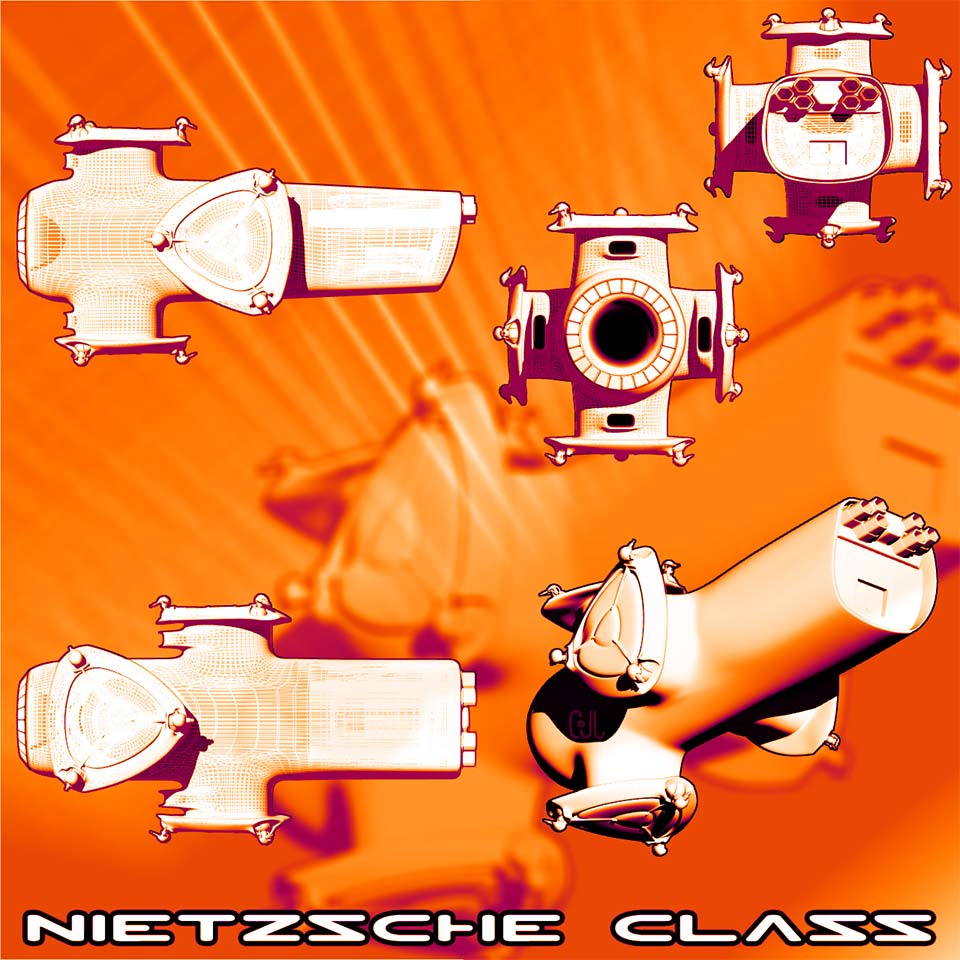
\includegraphics[width=\textwidth]{../images/vessels/NietzscheSchematics.jpg}
}
    \caption{A translated version of the above visual description for the Andolian Protectorate's Nietzsche capital vessel.}
    \label{fig:vessel-nietsche}
\end{center}
\end{figure}




% LocalWords:  Aerans Aeran Artstyle Aera Pinnace Acrotatus Agasicles Agesilaus
% LocalWords:  Agesipolis Agis Alcmenes Anaxander Wiki Anaxandridas Rlaan Areus
% LocalWords:  Anaxidamus Ariston Charillus Cleombrotus Cleomenes Demaratus Uln
% LocalWords:  Theopompus Dorissus Echestratus Eurycratides Eurypon Leons Bzbr
% LocalWords:  Nicander Pausanias Pleistarchus UnAeranned Pleistoanax Andolian
% LocalWords:  Spaceborn's MacGyver Polydectes Polydorus EVAs Procles Prytanis
% LocalWords:  Soos Teleclus terraforming Aenethforming Zeuxidamus homeworld
% LocalWords:  coreward chemoreception Klk'k Aeneth ecologies Shmrn

\section{Portfolio: The Bzbr}
Ships overview for all groups (Work In Progress): \href{http://vegastrike.sourceforge.net/wiki/Artstyle\_guide:Overview\_Guide}{Ship Overview} \\
Art-style Guide (Work In Progress): \href{http://vegastrike.sourceforge.net/wiki/Artstyle\_guide:Bzbr}{Artstyle Guide} \\
Species overview: \href{http://vegastrike.sourceforge.net/wiki/Species:Humanity}{Species:Bzbr} \\

\subsection{Origin}
\begin{itemize}
\item Sector: 
\item System: 
\item Origin Planet:  
\item Gravity: 

\item Atmosphere: 

\item Primary liquid bodies: 

\item Average temperature of homeworld (pre-industrialization):

\item Sun: 

\item Primary challenges (pre-industrialization): 
\end{itemize}

%ORIGIN COMMENTS GO HERE

\subsubsection{Habitat}

\subsection{Physical}
\begin{itemize}
\item Dimensions: 

\item Mass: 

\item Skeletal system: 

\item Major divisions: 

\item Senses: 

\item Visual acuity: 

\item Chemosense: 

\item Locomotion: 

\item Manipulators: 

\item Textural appearance: 
\end{itemize}

%PHYSICAL COMMENTS GO HERE

\subsection{Mental}


\subsection{Technological}
\begin{itemize}
\item Tech: 


\item Weapons:

\item Tactics:
\begin{itemize}
\item    Small groups: 
\item    Large groups/Fleets: 
\end{itemize}


\item Installations:


\end{itemize}

\subsection{Culture}

\subsubsection{Factions and Organizational Groups}
Listed below are noteworthy Aeran sub-factions and organizational groups: 
\begin{itemize}
\item FACTIONS GO HERE
\end{itemize}

\subsubsection{Religion}

\subsubsection{Cultural Aesthetics}

\subsection{Writing, numbers, and insignia}

\subsection{Faction: PRIMARY FACTION}
%Faction data 
%Aera 
%Species 	Aera 
%Homeworld (Origin) 	Aeneth 
%Capital 	Aeneth 


\subsubsection{A Brief History of the PRIMARY FACTION}


\subsubsection{Development}

\subsubsection{Culture}

\subsubsection{Organization}

\subsection{Faction: OTHER FACTIONS}

%Faction data 
%Merchant Marines 
%Species 	Aera 
%Homeworld (Origin) 	Aeneth 
%Capital 	Aeneth 


\subsection{Vessels}

\subsubsection{Style Overview}
\begin{itemize}

\item Primary distinguishing color ranges: 

\item Common accent colors:

\item Primary lighting color:

\item Frequently visible: 

\item Rarely visible:

\item Seen inside, but not out: 

\item Moving parts(non-turret): 

\item Capital vs. light craft: 

\end{itemize}

\subsubsection{Surface features of large vessels}

\subsubsection{Small things found on the hull of a large  vessel}
\begin{itemize}
\item Service/Maintenance hatches
\end{itemize}
{\it Somewhat larger things found on the hull of a large Aeran vessel:}
\begin{itemize}
\item Escape pod launcher ports
\end{itemize}
{\it Yet larger things ... :}
\begin{itemize}
\item Pinnace/lander launch bay (non-carrier vessels)
\end{itemize}

\subsubsection{Listing of vessels}

\begin{itemize}
\item \href{http://vegastrike.sourceforge.net/wiki/Vessel:FOO}{FOO:} 

Existing concept art is not particularly canonical. Please redesign.

\end{itemize}

% LocalWords:  Aerans Aeran Artstyle Aera Pinnace Acrotatus Agasicles Agesilaus
% LocalWords:  Agesipolis Agis Alcmenes Anaxander Wiki Anaxandridas Rlaan Areus
% LocalWords:  Anaxidamus Ariston Charillus Cleombrotus Cleomenes Demaratus Uln
% LocalWords:  Theopompus Dorissus Echestratus Eurycratides Eurypon Leons Bzbr
% LocalWords:  Nicander Pausanias Pleistarchus UnAeranned Pleistoanax Andolian
% LocalWords:  Spaceborn's MacGyver Polydectes Polydorus EVAs Procles Prytanis
% LocalWords:  Soos Teleclus terraforming Aenethforming Zeuxidamus homeworld
% LocalWords:  coreward chemoreception Klk'k Aeneth ecologies Shmrn

\section{Portfolio: The Confederation of Inhabited Worlds}
Ships overview for all groups (Work In Progress): \href{http://vegastrike.sourceforge.net/wiki/Artstyle\_guide:Overview\_Guide}{Ship Overview} \\
Art-style Guide (Work In Progress): \href{http://vegastrike.sourceforge.net/wiki/Artstyle\_guide:Confederation}{Artstyle Guide} \\
Species overviews: \href{http://vegastrike.sourceforge.net/wiki/Species:Humanity}{Species:Humanity} \\
\href{http://vegastrike.sourceforge.net/wiki/Species:Klk\'k}{Species:Klk\'k} \\
\href{http://vegastrike.sourceforge.net/wiki/Species:Purth}{Species:Purth} \\
\href{http://vegastrike.sourceforge.net/wiki/Species:Mishtali}{Species:Mishtali} \\
\href{http://vegastrike.sourceforge.net/wiki/Species:Dgn}{Species:Dgn} \\

\subsection{Origin}
\begin{itemize}
\item Gravity: 

\item Atmosphere: 

\item Primary liquid bodies: 

\item Average temperature of homeworld (pre-industrialization):

\item Sun: 

\item Primary challenges (pre-industrialization): 
\end{itemize}

%ORIGIN COMMENTS GO HERE

\subsubsection{Habitat}

\subsection{Physical}
\begin{itemize}
\item Dimensions: 

\item Mass: 

\item Skeletal system: 

\item Major divisions: 

\item Senses: 

\item Visual acuity: 

\item Chemosense: 

\item Locomotion: 

\item Manipulators: 

\item Textural appearance: 
\end{itemize}

%PHYSICAL COMMENTS GO HERE

\subsection{Mental}


\subsection{Technological}
\begin{itemize}
\item Tech: 


\item Weapons:

\item Tactics:
\begin{itemize}
\item    Small groups: 
\item    Large groups/Fleets: 
\end{itemize}


\item Installations:


\end{itemize}

\subsection{Culture}

\subsubsection{Factions and Organizational Groups}
Listed below are noteworthy Aeran sub-factions and organizational groups: 
\begin{itemize}
\item FACTIONS GO HERE
\end{itemize}

\subsubsection{Religion}

\subsubsection{Cultural Aesthetics}

\subsection{Writing, numbers, and insignia}

\subsection{Faction: PRIMARY FACTION}
%Faction data 
%Aera 
%Species 	Aera 
%Homeworld (Origin) 	Aeneth 
%Capital 	Aeneth 


\subsubsection{A Brief History of the PRIMARY FACTION}


\subsubsection{Development}

\subsubsection{Culture}

\subsubsection{Organization}

\subsection{Faction: OTHER FACTIONS}

%Faction data 
%Merchant Marines 
%Species 	Aera 
%Homeworld (Origin) 	Aeneth 
%Capital 	Aeneth 


\subsection{Vessels}

\subsubsection{Style Overview}
\begin{itemize}

\item Primary distinguishing color ranges: 

\item Common accent colors:

\item Primary lighting color:

\item Frequently visible: 

\item Rarely visible:

\item Seen inside, but not out: 

\item Moving parts(non-turret): 

\item Capital vs. light craft: 

\end{itemize}

\subsubsection{Surface features of large vessels}

\subsubsection{Small things found on the hull of a large  vessel}
\begin{itemize}
\item Service/Maintenance hatches
\end{itemize}
{\it Somewhat larger things found on the hull of a large Aeran vessel:}
\begin{itemize}
\item Escape pod launcher ports
\end{itemize}
{\it Yet larger things ... :}
\begin{itemize}
\item Pinnace/lander launch bay (non-carrier vessels)
\end{itemize}

\subsubsection{Listing of vessels}

\begin{itemize}
\item \href{http://vegastrike.sourceforge.net/wiki/Vessel:FOO}{FOO:} 

Existing concept art is not particularly canonical. Please redesign.

\end{itemize}

% LocalWords:  Aerans Aeran Artstyle Aera Pinnace Acrotatus Agasicles Agesilaus
% LocalWords:  Agesipolis Agis Alcmenes Anaxander Wiki Anaxandridas Rlaan Areus
% LocalWords:  Anaxidamus Ariston Charillus Cleombrotus Cleomenes Demaratus Uln
% LocalWords:  Theopompus Dorissus Echestratus Eurycratides Eurypon Leons Bzbr
% LocalWords:  Nicander Pausanias Pleistarchus UnAeranned Pleistoanax Andolian
% LocalWords:  Spaceborn's MacGyver Polydectes Polydorus EVAs Procles Prytanis
% LocalWords:  Soos Teleclus terraforming Aenethforming Zeuxidamus homeworld
% LocalWords:  coreward chemoreception Klk'k Aeneth ecologies Shmrn
     
\section{Portfolio: Criminal Elements}
Ships overview for all groups (Work In Progress): \href{http://vegastrike.sourceforge.net/wiki/Artstyle\_guide:Overview\_Guide}{Ship Overview} \\
Art-style Guide (Work In Progress): \href{http://vegastrike.sourceforge.net/wiki/Artstyle\_guide:Pirates}{Artstyle Guide} \\


\subsection{Origin}
\begin{itemize}
\item Gravity: 

\item Atmosphere: 

\item Primary liquid bodies: 

\item Average temperature of homeworld (pre-industrialization):

\item Sun: 

\item Primary challenges (pre-industrialization): 
\end{itemize}

%ORIGIN COMMENTS GO HERE

\subsubsection{Habitat}

\subsection{Physical}
\begin{itemize}
\item Dimensions: 

\item Mass: 

\item Skeletal system: 

\item Major divisions: 

\item Senses: 

\item Visual acuity: 

\item Chemosense: 

\item Locomotion: 

\item Manipulators: 

\item Textural appearance: 
\end{itemize}

%PHYSICAL COMMENTS GO HERE

\subsection{Mental}


\subsection{Technological}
\begin{itemize}
\item Tech: 


\item Weapons:

\item Tactics:
\begin{itemize}
\item    Small groups: 
\item    Large groups/Fleets: 
\end{itemize}


\item Installations:


\end{itemize}

\subsection{Culture}

\subsubsection{Factions and Organizational Groups}
Listed below are noteworthy Aeran sub-factions and organizational groups: 
\begin{itemize}
\item FACTIONS GO HERE
\end{itemize}

\subsubsection{Religion}

\subsubsection{Cultural Aesthetics}

\subsection{Writing, numbers, and insignia}

\subsection{Faction: PRIMARY FACTION}
%Faction data 
%Aera 
%Species 	Aera 
%Homeworld (Origin) 	Aeneth 
%Capital 	Aeneth 


\subsubsection{A Brief History of the PRIMARY FACTION}


\subsubsection{Development}

\subsubsection{Culture}

\subsubsection{Organization}

\subsection{Faction: OTHER FACTIONS}

%Faction data 
%Merchant Marines 
%Species 	Aera 
%Homeworld (Origin) 	Aeneth 
%Capital 	Aeneth 


\subsection{Vessels}

\subsubsection{Style Overview}
\begin{itemize}

\item Primary distinguishing color ranges: 

\item Common accent colors:

\item Primary lighting color:

\item Frequently visible: 

\item Rarely visible:

\item Seen inside, but not out: 

\item Moving parts(non-turret): 

\item Capital vs. light craft: 

\end{itemize}

\subsubsection{Surface features of large vessels}

\subsubsection{Small things found on the hull of a large  vessel}
\begin{itemize}
\item Service/Maintenance hatches
\end{itemize}
{\it Somewhat larger things found on the hull of a large Aeran vessel:}
\begin{itemize}
\item Escape pod launcher ports
\end{itemize}
{\it Yet larger things ... :}
\begin{itemize}
\item Pinnace/lander launch bay (non-carrier vessels)
\end{itemize}

\subsubsection{Listing of vessels}

\begin{itemize}
\item \href{http://vegastrike.sourceforge.net/wiki/Vessel:FOO}{FOO:} 

Existing concept art is not particularly canonical. Please redesign.

\end{itemize}

% LocalWords:  Aerans Aeran Artstyle Aera Pinnace Acrotatus Agasicles Agesilaus
% LocalWords:  Agesipolis Agis Alcmenes Anaxander Wiki Anaxandridas Rlaan Areus
% LocalWords:  Anaxidamus Ariston Charillus Cleombrotus Cleomenes Demaratus Uln
% LocalWords:  Theopompus Dorissus Echestratus Eurycratides Eurypon Leons Bzbr
% LocalWords:  Nicander Pausanias Pleistarchus UnAeranned Pleistoanax Andolian
% LocalWords:  Spaceborn's MacGyver Polydectes Polydorus EVAs Procles Prytanis
% LocalWords:  Soos Teleclus terraforming Aenethforming Zeuxidamus homeworld
% LocalWords:  coreward chemoreception Klk'k Aeneth ecologies Shmrn

\section{Portfolio: The Dgn}
Ships overview for all groups (Work In Progress): \href{http://vegastrike.sourceforge.net/wiki/Artstyle\_guide:Overview\_Guide}{Ship Overview} \\
Art-style Guide (Work In Progress): \href{http://vegastrike.sourceforge.net/wiki/Artstyle\_guide:Dgn}{Artstyle Guide} \\
Species overview: \href{http://vegastrike.sourceforge.net/wiki/Species:Dgn}{Species:Dgn} \\

\subsection{Origin}
\begin{itemize}
\item Sector: 
\item System: 
\item Origin Planet:  
\item Gravity: 

\item Atmosphere: 

\item Primary liquid bodies: 

\item Average temperature of homeworld (pre-industrialization):

\item Sun: 

\item Primary challenges (pre-industrialization): 
\end{itemize}

%ORIGIN COMMENTS GO HERE

\subsubsection{Habitat}

\subsection{Physical}
\begin{itemize}
\item Dimensions: 

\item Mass: 

\item Skeletal system: 

\item Major divisions: 

\item Senses: 

\item Visual acuity: 

\item Chemosense: 

\item Locomotion: 

\item Manipulators: 

\item Textural appearance: 
\end{itemize}

%PHYSICAL COMMENTS GO HERE

\subsection{Mental}


\subsection{Technological}
\begin{itemize}
\item Tech: 


\item Weapons:

\item Tactics:
\begin{itemize}
\item    Small groups: 
\item    Large groups/Fleets: 
\end{itemize}


\item Installations:


\end{itemize}

\subsection{Culture}

\subsubsection{Factions and Organizational Groups}
Listed below are noteworthy Aeran sub-factions and organizational groups: 
\begin{itemize}
\item FACTIONS GO HERE
\end{itemize}

\subsubsection{Religion}

\subsubsection{Cultural Aesthetics}

\subsection{Writing, numbers, and insignia}

\subsection{Faction: PRIMARY FACTION}
%Faction data 
%Aera 
%Species 	Aera 
%Homeworld (Origin) 	Aeneth 
%Capital 	Aeneth 


\subsubsection{A Brief History of the PRIMARY FACTION}


\subsubsection{Development}

\subsubsection{Culture}

\subsubsection{Organization}

\subsection{Faction: OTHER FACTIONS}

%Faction data 
%Merchant Marines 
%Species 	Aera 
%Homeworld (Origin) 	Aeneth 
%Capital 	Aeneth 


\subsection{Vessels}

\subsubsection{Style Overview}
\begin{itemize}

\item Primary distinguishing color ranges: 

\item Common accent colors:

\item Primary lighting color:

\item Frequently visible: 

\item Rarely visible:

\item Seen inside, but not out: 

\item Moving parts(non-turret): 

\item Capital vs. light craft: 

\end{itemize}

\subsubsection{Surface features of large vessels}

\subsubsection{Small things found on the hull of a large  vessel}
\begin{itemize}
\item Service/Maintenance hatches
\end{itemize}
{\it Somewhat larger things found on the hull of a large Aeran vessel:}
\begin{itemize}
\item Escape pod launcher ports
\end{itemize}
{\it Yet larger things ... :}
\begin{itemize}
\item Pinnace/lander launch bay (non-carrier vessels)
\end{itemize}

\subsubsection{Listing of vessels}

\begin{itemize}
\item \href{http://vegastrike.sourceforge.net/wiki/Vessel:FOO}{FOO:} 

Existing concept art is not particularly canonical. Please redesign.

\end{itemize}

% LocalWords:  Aerans Aeran Artstyle Aera Pinnace Acrotatus Agasicles Agesilaus
% LocalWords:  Agesipolis Agis Alcmenes Anaxander Wiki Anaxandridas Rlaan Areus
% LocalWords:  Anaxidamus Ariston Charillus Cleombrotus Cleomenes Demaratus Uln
% LocalWords:  Theopompus Dorissus Echestratus Eurycratides Eurypon Leons Bzbr
% LocalWords:  Nicander Pausanias Pleistarchus UnAeranned Pleistoanax Andolian
% LocalWords:  Spaceborn's MacGyver Polydectes Polydorus EVAs Procles Prytanis
% LocalWords:  Soos Teleclus terraforming Aenethforming Zeuxidamus homeworld
% LocalWords:  coreward chemoreception Klk'k Aeneth ecologies Shmrn
             
\section{Portfolio: The Forsaken (Union of Dispossessed Settlers)}
Ships overview for all groups (Work In Progress): \href{http://vegastrike.sourceforge.net/wiki/Artstyle\_guide:Overview\_Guide}{Ship Overview} \\
Art-style Guide (Work In Progress): \href{http://vegastrike.sourceforge.net/wiki/Artstyle\_guide:Forsaken}{Artstyle Guide} \\
Species overview: \href{http://vegastrike.sourceforge.net/wiki/Species:Humanity}{Species:Humanity} \\

\subsection{Origin}
\begin{itemize}
\item Sector: 
\item System: 
\item Origin Planet:  
\item Gravity: 

\item Atmosphere: 

\item Primary liquid bodies: 

\item Average temperature of homeworld (pre-industrialization):

\item Sun: 

\item Primary challenges (pre-industrialization): 
\end{itemize}

%ORIGIN COMMENTS GO HERE

\subsubsection{Habitat}

\subsection{Physical}
\begin{itemize}
\item Dimensions: 

\item Mass: 

\item Skeletal system: 

\item Major divisions: 

\item Senses: 

\item Visual acuity: 

\item Chemosense: 

\item Locomotion: 

\item Manipulators: 

\item Textural appearance: 
\end{itemize}

%PHYSICAL COMMENTS GO HERE

\subsection{Mental}


\subsection{Technological}
\begin{itemize}
\item Tech: 


\item Weapons:

\item Tactics:
\begin{itemize}
\item    Small groups: 
\item    Large groups/Fleets: 
\end{itemize}


\item Installations:


\end{itemize}

\subsection{Culture}

\subsubsection{Factions and Organizational Groups}
Listed below are noteworthy Aeran sub-factions and organizational groups: 
\begin{itemize}
\item FACTIONS GO HERE
\end{itemize}

\subsubsection{Religion}

\subsubsection{Cultural Aesthetics}

\subsection{Writing, numbers, and insignia}

\subsection{Faction: PRIMARY FACTION}
%Faction data 
%Aera 
%Species 	Aera 
%Homeworld (Origin) 	Aeneth 
%Capital 	Aeneth 


\subsubsection{A Brief History of the PRIMARY FACTION}


\subsubsection{Development}

\subsubsection{Culture}

\subsubsection{Organization}

\subsection{Faction: OTHER FACTIONS}

%Faction data 
%Merchant Marines 
%Species 	Aera 
%Homeworld (Origin) 	Aeneth 
%Capital 	Aeneth 


\subsection{Vessels}

\subsubsection{Style Overview}
\begin{itemize}

\item Primary distinguishing color ranges: 

\item Common accent colors:

\item Primary lighting color:

\item Frequently visible: 

\item Rarely visible:

\item Seen inside, but not out: 

\item Moving parts(non-turret): 

\item Capital vs. light craft: 

\end{itemize}

\subsubsection{Surface features of large vessels}

\subsubsection{Small things found on the hull of a large  vessel}
\begin{itemize}
\item Service/Maintenance hatches
\end{itemize}
{\it Somewhat larger things found on the hull of a large Aeran vessel:}
\begin{itemize}
\item Escape pod launcher ports
\end{itemize}
{\it Yet larger things ... :}
\begin{itemize}
\item Pinnace/lander launch bay (non-carrier vessels)
\end{itemize}

\subsubsection{Listing of vessels}

\begin{itemize}
\item \href{http://vegastrike.sourceforge.net/wiki/Vessel:FOO}{FOO:} 

Existing concept art is not particularly canonical. Please redesign.

\end{itemize}

% LocalWords:  Aerans Aeran Artstyle Aera Pinnace Acrotatus Agasicles Agesilaus
% LocalWords:  Agesipolis Agis Alcmenes Anaxander Wiki Anaxandridas Rlaan Areus
% LocalWords:  Anaxidamus Ariston Charillus Cleombrotus Cleomenes Demaratus Uln
% LocalWords:  Theopompus Dorissus Echestratus Eurycratides Eurypon Leons Bzbr
% LocalWords:  Nicander Pausanias Pleistarchus UnAeranned Pleistoanax Andolian
% LocalWords:  Spaceborn's MacGyver Polydectes Polydorus EVAs Procles Prytanis
% LocalWords:  Soos Teleclus terraforming Aenethforming Zeuxidamus homeworld
% LocalWords:  coreward chemoreception Klk'k Aeneth ecologies Shmrn
             
\section{Portfolio: The Highborn}
Ships overview for all groups (Work In Progress): \href{http://vegastrike.sourceforge.net/wiki/Artstyle\_guide:Overview\_Guide}{Ship Overview} \\
Art-style Guide (Work In Progress): \href{http://vegastrike.sourceforge.net/wiki/Artstyle\_guide:Highborn}{Artstyle Guide} \\
Species overview: \href{http://vegastrike.sourceforge.net/wiki/Species:Humanity}{Species:Humanity} \\

\subsection{Origin}
\begin{itemize}
\item Sector: 
\item System: 
\item Origin Planet:  
\item Gravity: 

\item Atmosphere: 

\item Primary liquid bodies: 

\item Average temperature of homeworld (pre-industrialization):

\item Sun: 

\item Primary challenges (pre-industrialization): 
\end{itemize}

%ORIGIN COMMENTS GO HERE

\subsubsection{Habitat}

\subsection{Physical}
\begin{itemize}
\item Dimensions: 

\item Mass: 

\item Skeletal system: 

\item Major divisions: 

\item Senses: 

\item Visual acuity: 

\item Chemosense: 

\item Locomotion: 

\item Manipulators: 

\item Textural appearance: 
\end{itemize}

%PHYSICAL COMMENTS GO HERE

\subsection{Mental}


\subsection{Technological}
\begin{itemize}
\item Tech: 


\item Weapons:

\item Tactics:
\begin{itemize}
\item    Small groups: 
\item    Large groups/Fleets: 
\end{itemize}


\item Installations:


\end{itemize}

\subsection{Culture}

\subsubsection{Factions and Organizational Groups}
Listed below are noteworthy Aeran sub-factions and organizational groups: 
\begin{itemize}
\item FACTIONS GO HERE
\end{itemize}

\subsubsection{Religion}

\subsubsection{Cultural Aesthetics}

\subsection{Writing, numbers, and insignia}

\subsection{Faction: PRIMARY FACTION}
%Faction data 
%Aera 
%Species 	Aera 
%Homeworld (Origin) 	Aeneth 
%Capital 	Aeneth 


\subsubsection{A Brief History of the PRIMARY FACTION}


\subsubsection{Development}

\subsubsection{Culture}

\subsubsection{Organization}

\subsection{Faction: OTHER FACTIONS}

%Faction data 
%Merchant Marines 
%Species 	Aera 
%Homeworld (Origin) 	Aeneth 
%Capital 	Aeneth 


\subsection{Vessels}

\subsubsection{Style Overview}
\begin{itemize}

\item Primary distinguishing color ranges: 

\item Common accent colors:

\item Primary lighting color:

\item Frequently visible: 

\item Rarely visible:

\item Seen inside, but not out: 

\item Moving parts(non-turret): 

\item Capital vs. light craft: 

\end{itemize}

\subsubsection{Surface features of large vessels}

\subsubsection{Small things found on the hull of a large  vessel}
\begin{itemize}
\item Service/Maintenance hatches
\end{itemize}
{\it Somewhat larger things found on the hull of a large Aeran vessel:}
\begin{itemize}
\item Escape pod launcher ports
\end{itemize}
{\it Yet larger things ... :}
\begin{itemize}
\item Pinnace/lander launch bay (non-carrier vessels)
\end{itemize}

\subsubsection{Listing of vessels}

\begin{itemize}
\item \href{http://vegastrike.sourceforge.net/wiki/Vessel:FOO}{FOO:} 

Existing concept art is not particularly canonical. Please redesign.

\end{itemize}

% LocalWords:  Aerans Aeran Artstyle Aera Pinnace Acrotatus Agasicles Agesilaus
% LocalWords:  Agesipolis Agis Alcmenes Anaxander Wiki Anaxandridas Rlaan Areus
% LocalWords:  Anaxidamus Ariston Charillus Cleombrotus Cleomenes Demaratus Uln
% LocalWords:  Theopompus Dorissus Echestratus Eurycratides Eurypon Leons Bzbr
% LocalWords:  Nicander Pausanias Pleistarchus UnAeranned Pleistoanax Andolian
% LocalWords:  Spaceborn's MacGyver Polydectes Polydorus EVAs Procles Prytanis
% LocalWords:  Soos Teleclus terraforming Aenethforming Zeuxidamus homeworld
% LocalWords:  coreward chemoreception Klk'k Aeneth ecologies Shmrn
     
\section{Portfolio: Homeland Security}
Ships overview for all groups (Work In Progress): \href{http://vegastrike.sourceforge.net/wiki/Artstyle\_guide:Overview\_Guide}{Ship Overview} \\
Art-style Guide (Work In Progress): \href{http://vegastrike.sourceforge.net/wiki/Artstyle\_guide:Homeland\_Security}{Artstyle Guide} \\
Species overview: \href{http://vegastrike.sourceforge.net/wiki/Species:Humanity}{Species:Humanity} \\

\subsection{Origin}
\begin{itemize}
\item Gravity: 

\item Atmosphere: 

\item Primary liquid bodies: 

\item Average temperature of homeworld (pre-industrialization):

\item Sun: 

\item Primary challenges (pre-industrialization): 
\end{itemize}

%ORIGIN COMMENTS GO HERE

\subsubsection{Habitat}

\subsection{Physical}
\begin{itemize}
\item Dimensions: 

\item Mass: 

\item Skeletal system: 

\item Major divisions: 

\item Senses: 

\item Visual acuity: 

\item Chemosense: 

\item Locomotion: 

\item Manipulators: 

\item Textural appearance: 
\end{itemize}

%PHYSICAL COMMENTS GO HERE

\subsection{Mental}


\subsection{Technological}
\begin{itemize}
\item Tech: 


\item Weapons:

\item Tactics:
\begin{itemize}
\item    Small groups: 
\item    Large groups/Fleets: 
\end{itemize}


\item Installations:


\end{itemize}

\subsection{Culture}

\subsubsection{Factions and Organizational Groups}
Listed below are noteworthy Aeran sub-factions and organizational groups: 
\begin{itemize}
\item FACTIONS GO HERE
\end{itemize}

\subsubsection{Religion}

\subsubsection{Cultural Aesthetics}

\subsection{Writing, numbers, and insignia}

\subsection{Faction: PRIMARY FACTION}
%Faction data 
%Aera 
%Species 	Aera 
%Homeworld (Origin) 	Aeneth 
%Capital 	Aeneth 


\subsubsection{A Brief History of the PRIMARY FACTION}


\subsubsection{Development}

\subsubsection{Culture}

\subsubsection{Organization}

\subsection{Faction: OTHER FACTIONS}

%Faction data 
%Merchant Marines 
%Species 	Aera 
%Homeworld (Origin) 	Aeneth 
%Capital 	Aeneth 


\subsection{Vessels}

\subsubsection{Style Overview}
\begin{itemize}

\item Primary distinguishing color ranges: 

\item Common accent colors:

\item Primary lighting color:

\item Frequently visible: 

\item Rarely visible:

\item Seen inside, but not out: 

\item Moving parts(non-turret): 

\item Capital vs. light craft: 

\end{itemize}

\subsubsection{Surface features of large vessels}

\subsubsection{Small things found on the hull of a large  vessel}
\begin{itemize}
\item Service/Maintenance hatches
\end{itemize}
{\it Somewhat larger things found on the hull of a large Aeran vessel:}
\begin{itemize}
\item Escape pod launcher ports
\end{itemize}
{\it Yet larger things ... :}
\begin{itemize}
\item Pinnace/lander launch bay (non-carrier vessels)
\end{itemize}

\subsubsection{Listing of vessels}

\begin{itemize}
\item \href{http://vegastrike.sourceforge.net/wiki/Vessel:FOO}{FOO:} 

Existing concept art is not particularly canonical. Please redesign.

\end{itemize}

% LocalWords:  Aerans Aeran Artstyle Aera Pinnace Acrotatus Agasicles Agesilaus
% LocalWords:  Agesipolis Agis Alcmenes Anaxander Wiki Anaxandridas Rlaan Areus
% LocalWords:  Anaxidamus Ariston Charillus Cleombrotus Cleomenes Demaratus Uln
% LocalWords:  Theopompus Dorissus Echestratus Eurycratides Eurypon Leons Bzbr
% LocalWords:  Nicander Pausanias Pleistarchus UnAeranned Pleistoanax Andolian
% LocalWords:  Spaceborn's MacGyver Polydectes Polydorus EVAs Procles Prytanis
% LocalWords:  Soos Teleclus terraforming Aenethforming Zeuxidamus homeworld
% LocalWords:  coreward chemoreception Klk'k Aeneth ecologies Shmrn

\section{Portfolio: The Bounty Hunter's Guild}
Ships overview for all groups (Work In Progress): \href{http://vegastrike.sourceforge.net/wiki/Artstyle\_guide:Overview\_Guide}{Ship Overview} \\
Art-style Guide (Work In Progress): \href{http://vegastrike.sourceforge.net/wiki/Artstyle\_guide:Hunters}{Artstyle Guide} \\
Species overview: \href{http://vegastrike.sourceforge.net/wiki/Species:Humanity}{Species:Humanity} \\

\subsection{Origin}
\begin{itemize}
\item Gravity: 

\item Atmosphere: 

\item Primary liquid bodies: 

\item Average temperature of homeworld (pre-industrialization):

\item Sun: 

\item Primary challenges (pre-industrialization): 
\end{itemize}

%ORIGIN COMMENTS GO HERE

\subsubsection{Habitat}

\subsection{Physical}
\begin{itemize}
\item Dimensions: 

\item Mass: 

\item Skeletal system: 

\item Major divisions: 

\item Senses: 

\item Visual acuity: 

\item Chemosense: 

\item Locomotion: 

\item Manipulators: 

\item Textural appearance: 
\end{itemize}

%PHYSICAL COMMENTS GO HERE

\subsection{Mental}


\subsection{Technological}
\begin{itemize}
\item Tech: 


\item Weapons:

\item Tactics:
\begin{itemize}
\item    Small groups: 
\item    Large groups/Fleets: 
\end{itemize}


\item Installations:


\end{itemize}

\subsection{Culture}

\subsubsection{Factions and Organizational Groups}
Listed below are noteworthy Aeran sub-factions and organizational groups: 
\begin{itemize}
\item FACTIONS GO HERE
\end{itemize}

\subsubsection{Religion}

\subsubsection{Cultural Aesthetics}

\subsection{Writing, numbers, and insignia}

\subsection{Faction: PRIMARY FACTION}
%Faction data 
%Aera 
%Species 	Aera 
%Homeworld (Origin) 	Aeneth 
%Capital 	Aeneth 


\subsubsection{A Brief History of the PRIMARY FACTION}


\subsubsection{Development}

\subsubsection{Culture}

\subsubsection{Organization}

\subsection{Faction: OTHER FACTIONS}

%Faction data 
%Merchant Marines 
%Species 	Aera 
%Homeworld (Origin) 	Aeneth 
%Capital 	Aeneth 


\subsection{Vessels}

\subsubsection{Style Overview}
\begin{itemize}

\item Primary distinguishing color ranges: 

\item Common accent colors:

\item Primary lighting color:

\item Frequently visible: 

\item Rarely visible:

\item Seen inside, but not out: 

\item Moving parts(non-turret): 

\item Capital vs. light craft: 

\end{itemize}

\subsubsection{Surface features of large vessels}

\subsubsection{Small things found on the hull of a large  vessel}
\begin{itemize}
\item Service/Maintenance hatches
\end{itemize}
{\it Somewhat larger things found on the hull of a large Aeran vessel:}
\begin{itemize}
\item Escape pod launcher ports
\end{itemize}
{\it Yet larger things ... :}
\begin{itemize}
\item Pinnace/lander launch bay (non-carrier vessels)
\end{itemize}

\subsubsection{Listing of vessels}

\begin{itemize}
\item \href{http://vegastrike.sourceforge.net/wiki/Vessel:FOO}{FOO:} 

Existing concept art is not particularly canonical. Please redesign.

\end{itemize}

% LocalWords:  Aerans Aeran Artstyle Aera Pinnace Acrotatus Agasicles Agesilaus
% LocalWords:  Agesipolis Agis Alcmenes Anaxander Wiki Anaxandridas Rlaan Areus
% LocalWords:  Anaxidamus Ariston Charillus Cleombrotus Cleomenes Demaratus Uln
% LocalWords:  Theopompus Dorissus Echestratus Eurycratides Eurypon Leons Bzbr
% LocalWords:  Nicander Pausanias Pleistarchus UnAeranned Pleistoanax Andolian
% LocalWords:  Spaceborn's MacGyver Polydectes Polydorus EVAs Procles Prytanis
% LocalWords:  Soos Teleclus terraforming Aenethforming Zeuxidamus homeworld
% LocalWords:  coreward chemoreception Klk'k Aeneth ecologies Shmrn

\section{Portfolio: The Interstellar Shipping and Mercantile Guild}
Ships overview for all groups (Work In Progress): \href{http://vegastrike.sourceforge.net/wiki/Artstyle\_guide:Overview\_Guide}{Ship Overview} \\
Art-style Guide (Work In Progress): \href{http://vegastrike.sourceforge.net/wiki/Artstyle\_guide:ISMG}{Artstyle Guide} \\
Species overview: \href{http://vegastrike.sourceforge.net/wiki/Species:Humanity}{Species:Humanity} \\

\subsection{Origin}
\begin{itemize}
\item Gravity: 

\item Atmosphere: 

\item Primary liquid bodies: 

\item Average temperature of homeworld (pre-industrialization):

\item Sun: 

\item Primary challenges (pre-industrialization): 
\end{itemize}

%ORIGIN COMMENTS GO HERE

\subsubsection{Habitat}

\subsection{Physical}
\begin{itemize}
\item Dimensions: 

\item Mass: 

\item Skeletal system: 

\item Major divisions: 

\item Senses: 

\item Visual acuity: 

\item Chemosense: 

\item Locomotion: 

\item Manipulators: 

\item Textural appearance: 
\end{itemize}

%PHYSICAL COMMENTS GO HERE

\subsection{Mental}


\subsection{Technological}
\begin{itemize}
\item Tech: 


\item Weapons:

\item Tactics:
\begin{itemize}
\item    Small groups: 
\item    Large groups/Fleets: 
\end{itemize}


\item Installations:


\end{itemize}

\subsection{Culture}

\subsubsection{Factions and Organizational Groups}
Listed below are noteworthy Aeran sub-factions and organizational groups: 
\begin{itemize}
\item FACTIONS GO HERE
\end{itemize}

\subsubsection{Religion}

\subsubsection{Cultural Aesthetics}

\subsection{Writing, numbers, and insignia}

\subsection{Faction: PRIMARY FACTION}
%Faction data 
%Aera 
%Species 	Aera 
%Homeworld (Origin) 	Aeneth 
%Capital 	Aeneth 


\subsubsection{A Brief History of the PRIMARY FACTION}


\subsubsection{Development}

\subsubsection{Culture}

\subsubsection{Organization}

\subsection{Faction: OTHER FACTIONS}

%Faction data 
%Merchant Marines 
%Species 	Aera 
%Homeworld (Origin) 	Aeneth 
%Capital 	Aeneth 


\subsection{Vessels}

\subsubsection{Style Overview}
\begin{itemize}

\item Primary distinguishing color ranges: 

\item Common accent colors:

\item Primary lighting color:

\item Frequently visible: 

\item Rarely visible:

\item Seen inside, but not out: 

\item Moving parts(non-turret): 

\item Capital vs. light craft: 

\end{itemize}

\subsubsection{Surface features of large vessels}

\subsubsection{Small things found on the hull of a large  vessel}
\begin{itemize}
\item Service/Maintenance hatches
\end{itemize}
{\it Somewhat larger things found on the hull of a large Aeran vessel:}
\begin{itemize}
\item Escape pod launcher ports
\end{itemize}
{\it Yet larger things ... :}
\begin{itemize}
\item Pinnace/lander launch bay (non-carrier vessels)
\end{itemize}

\subsubsection{Listing of vessels}

\begin{itemize}
\item \href{http://vegastrike.sourceforge.net/wiki/Vessel:FOO}{FOO:} 

Existing concept art is not particularly canonical. Please redesign.

\end{itemize}

% LocalWords:  Aerans Aeran Artstyle Aera Pinnace Acrotatus Agasicles Agesilaus
% LocalWords:  Agesipolis Agis Alcmenes Anaxander Wiki Anaxandridas Rlaan Areus
% LocalWords:  Anaxidamus Ariston Charillus Cleombrotus Cleomenes Demaratus Uln
% LocalWords:  Theopompus Dorissus Echestratus Eurycratides Eurypon Leons Bzbr
% LocalWords:  Nicander Pausanias Pleistarchus UnAeranned Pleistoanax Andolian
% LocalWords:  Spaceborn's MacGyver Polydectes Polydorus EVAs Procles Prytanis
% LocalWords:  Soos Teleclus terraforming Aenethforming Zeuxidamus homeworld
% LocalWords:  coreward chemoreception Klk'k Aeneth ecologies Shmrn
                  
\section{Portfolio: The Interstellar Socialist Organization}
Ships overview for all groups (Work In Progress): \href{http://vegastrike.sourceforge.net/wiki/Artstyle\_guide:Overview\_Guide}{Ship Overview} \\
Art-style Guide (Work In Progress): \href{http://vegastrike.sourceforge.net/wiki/Artstyle\_guide:ISO}{Artstyle Guide} \\
Species overview: \href{http://vegastrike.sourceforge.net/wiki/Species:Humanity}{Species:Humanity} \\

\subsection{Origin}
\begin{itemize}
\item Gravity: 

\item Atmosphere: 

\item Primary liquid bodies: 

\item Average temperature of homeworld (pre-industrialization):

\item Sun: 

\item Primary challenges (pre-industrialization): 
\end{itemize}

%ORIGIN COMMENTS GO HERE

\subsubsection{Habitat}

\subsection{Physical}
\begin{itemize}
\item Dimensions: 

\item Mass: 

\item Skeletal system: 

\item Major divisions: 

\item Senses: 

\item Visual acuity: 

\item Chemosense: 

\item Locomotion: 

\item Manipulators: 

\item Textural appearance: 
\end{itemize}

%PHYSICAL COMMENTS GO HERE

\subsection{Mental}


\subsection{Technological}
\begin{itemize}
\item Tech: 


\item Weapons:

\item Tactics:
\begin{itemize}
\item    Small groups: 
\item    Large groups/Fleets: 
\end{itemize}


\item Installations:


\end{itemize}

\subsection{Culture}

\subsubsection{Factions and Organizational Groups}
Listed below are noteworthy Aeran sub-factions and organizational groups: 
\begin{itemize}
\item FACTIONS GO HERE
\end{itemize}

\subsubsection{Religion}

\subsubsection{Cultural Aesthetics}

\subsection{Writing, numbers, and insignia}

\subsection{Faction: PRIMARY FACTION}
%Faction data 
%Aera 
%Species 	Aera 
%Homeworld (Origin) 	Aeneth 
%Capital 	Aeneth 


\subsubsection{A Brief History of the PRIMARY FACTION}


\subsubsection{Development}

\subsubsection{Culture}

\subsubsection{Organization}

\subsection{Faction: OTHER FACTIONS}

%Faction data 
%Merchant Marines 
%Species 	Aera 
%Homeworld (Origin) 	Aeneth 
%Capital 	Aeneth 


\subsection{Vessels}

\subsubsection{Style Overview}
\begin{itemize}

\item Primary distinguishing color ranges: 

\item Common accent colors:

\item Primary lighting color:

\item Frequently visible: 

\item Rarely visible:

\item Seen inside, but not out: 

\item Moving parts(non-turret): 

\item Capital vs. light craft: 

\end{itemize}

\subsubsection{Surface features of large vessels}

\subsubsection{Small things found on the hull of a large  vessel}
\begin{itemize}
\item Service/Maintenance hatches
\end{itemize}
{\it Somewhat larger things found on the hull of a large Aeran vessel:}
\begin{itemize}
\item Escape pod launcher ports
\end{itemize}
{\it Yet larger things ... :}
\begin{itemize}
\item Pinnace/lander launch bay (non-carrier vessels)
\end{itemize}

\subsubsection{Listing of vessels}

\begin{itemize}
\item \href{http://vegastrike.sourceforge.net/wiki/Vessel:FOO}{FOO:} 

Existing concept art is not particularly canonical. Please redesign.

\end{itemize}

% LocalWords:  Aerans Aeran Artstyle Aera Pinnace Acrotatus Agasicles Agesilaus
% LocalWords:  Agesipolis Agis Alcmenes Anaxander Wiki Anaxandridas Rlaan Areus
% LocalWords:  Anaxidamus Ariston Charillus Cleombrotus Cleomenes Demaratus Uln
% LocalWords:  Theopompus Dorissus Echestratus Eurycratides Eurypon Leons Bzbr
% LocalWords:  Nicander Pausanias Pleistarchus UnAeranned Pleistoanax Andolian
% LocalWords:  Spaceborn's MacGyver Polydectes Polydorus EVAs Procles Prytanis
% LocalWords:  Soos Teleclus terraforming Aenethforming Zeuxidamus homeworld
% LocalWords:  coreward chemoreception Klk'k Aeneth ecologies Shmrn
               
\section{Portfolio: The Klk\'k}
Ships overview for all groups (Work In Progress): \href{http://vegastrike.sourceforge.net/wiki/Artstyle\_guide:Overview\_Guide}{Ship Overview} \\
Art-style Guide (Work In Progress): \href{http://vegastrike.sourceforge.net/wiki/Artstyle\_guide:Klkk}{Artstyle Guide} \\
Species overview: \href{http://vegastrike.sourceforge.net/wiki/Species:Klkk}{Species:Klkk} \\

\subsection{Origin}
\begin{itemize}
\item Gravity: 

\item Atmosphere: 

\item Primary liquid bodies: 

\item Average temperature of homeworld (pre-industrialization):

\item Sun: 

\item Primary challenges (pre-industrialization): 
\end{itemize}

%ORIGIN COMMENTS GO HERE

\subsubsection{Habitat}

\subsection{Physical}
\begin{itemize}
\item Dimensions: 

\item Mass: 

\item Skeletal system: 

\item Major divisions: 

\item Senses: 

\item Visual acuity: 

\item Chemosense: 

\item Locomotion: 

\item Manipulators: 

\item Textural appearance: 
\end{itemize}

%PHYSICAL COMMENTS GO HERE

\subsection{Mental}


\subsection{Technological}
\begin{itemize}
\item Tech: 


\item Weapons:

\item Tactics:
\begin{itemize}
\item    Small groups: 
\item    Large groups/Fleets: 
\end{itemize}


\item Installations:


\end{itemize}

\subsection{Culture}

\subsubsection{Factions and Organizational Groups}
Listed below are noteworthy Aeran sub-factions and organizational groups: 
\begin{itemize}
\item FACTIONS GO HERE
\end{itemize}

\subsubsection{Religion}

\subsubsection{Cultural Aesthetics}

\subsection{Writing, numbers, and insignia}

\subsection{Faction: PRIMARY FACTION}
%Faction data 
%Aera 
%Species 	Aera 
%Homeworld (Origin) 	Aeneth 
%Capital 	Aeneth 


\subsubsection{A Brief History of the PRIMARY FACTION}


\subsubsection{Development}

\subsubsection{Culture}

\subsubsection{Organization}

\subsection{Faction: OTHER FACTIONS}

%Faction data 
%Merchant Marines 
%Species 	Aera 
%Homeworld (Origin) 	Aeneth 
%Capital 	Aeneth 


\subsection{Vessels}

\subsubsection{Style Overview}
\begin{itemize}

\item Primary distinguishing color ranges: 

\item Common accent colors:

\item Primary lighting color:

\item Frequently visible: 

\item Rarely visible:

\item Seen inside, but not out: 

\item Moving parts(non-turret): 

\item Capital vs. light craft: 

\end{itemize}

\subsubsection{Surface features of large vessels}

\subsubsection{Small things found on the hull of a large  vessel}
\begin{itemize}
\item Service/Maintenance hatches
\end{itemize}
{\it Somewhat larger things found on the hull of a large Aeran vessel:}
\begin{itemize}
\item Escape pod launcher ports
\end{itemize}
{\it Yet larger things ... :}
\begin{itemize}
\item Pinnace/lander launch bay (non-carrier vessels)
\end{itemize}

\subsubsection{Listing of vessels}

\begin{itemize}
\item \href{http://vegastrike.sourceforge.net/wiki/Vessel:FOO}{FOO:} 

Existing concept art is not particularly canonical. Please redesign.

\end{itemize}

% LocalWords:  Aerans Aeran Artstyle Aera Pinnace Acrotatus Agasicles Agesilaus
% LocalWords:  Agesipolis Agis Alcmenes Anaxander Wiki Anaxandridas Rlaan Areus
% LocalWords:  Anaxidamus Ariston Charillus Cleombrotus Cleomenes Demaratus Uln
% LocalWords:  Theopompus Dorissus Echestratus Eurycratides Eurypon Leons Bzbr
% LocalWords:  Nicander Pausanias Pleistarchus UnAeranned Pleistoanax Andolian
% LocalWords:  Spaceborn's MacGyver Polydectes Polydorus EVAs Procles Prytanis
% LocalWords:  Soos Teleclus terraforming Aenethforming Zeuxidamus homeworld
% LocalWords:  coreward chemoreception Klk'k Aeneth ecologies Shmrn
                 
\section{Portfolio: The League of Independent Human Worlds}
Ships overview for all groups (Work In Progress): \href{http://vegastrike.sourceforge.net/wiki/Artstyle\_guide:Overview\_Guide}{Ship Overview} \\
Art-style Guide (Work In Progress): \href{http://vegastrike.sourceforge.net/wiki/Artstyle\_guide:LIHW}{Artstyle Guide} \\
Species overview: \href{http://vegastrike.sourceforge.net/wiki/Species:Humanity}{Species:Humanity} \\

\subsection{Origin}
\begin{itemize}
\item Gravity: 

\item Atmosphere: 

\item Primary liquid bodies: 

\item Average temperature of homeworld (pre-industrialization):

\item Sun: 

\item Primary challenges (pre-industrialization): 
\end{itemize}

%ORIGIN COMMENTS GO HERE

\subsubsection{Habitat}

\subsection{Physical}
\begin{itemize}
\item Dimensions: 

\item Mass: 

\item Skeletal system: 

\item Major divisions: 

\item Senses: 

\item Visual acuity: 

\item Chemosense: 

\item Locomotion: 

\item Manipulators: 

\item Textural appearance: 
\end{itemize}

%PHYSICAL COMMENTS GO HERE

\subsection{Mental}


\subsection{Technological}
\begin{itemize}
\item Tech: 


\item Weapons:

\item Tactics:
\begin{itemize}
\item    Small groups: 
\item    Large groups/Fleets: 
\end{itemize}


\item Installations:


\end{itemize}

\subsection{Culture}

\subsubsection{Factions and Organizational Groups}
Listed below are noteworthy Aeran sub-factions and organizational groups: 
\begin{itemize}
\item FACTIONS GO HERE
\end{itemize}

\subsubsection{Religion}

\subsubsection{Cultural Aesthetics}

\subsection{Writing, numbers, and insignia}

\subsection{Faction: PRIMARY FACTION}
%Faction data 
%Aera 
%Species 	Aera 
%Homeworld (Origin) 	Aeneth 
%Capital 	Aeneth 


\subsubsection{A Brief History of the PRIMARY FACTION}


\subsubsection{Development}

\subsubsection{Culture}

\subsubsection{Organization}

\subsection{Faction: OTHER FACTIONS}

%Faction data 
%Merchant Marines 
%Species 	Aera 
%Homeworld (Origin) 	Aeneth 
%Capital 	Aeneth 


\subsection{Vessels}

\subsubsection{Style Overview}
\begin{itemize}

\item Primary distinguishing color ranges: 

\item Common accent colors:

\item Primary lighting color:

\item Frequently visible: 

\item Rarely visible:

\item Seen inside, but not out: 

\item Moving parts(non-turret): 

\item Capital vs. light craft: 

\end{itemize}

\subsubsection{Surface features of large vessels}

\subsubsection{Small things found on the hull of a large  vessel}
\begin{itemize}
\item Service/Maintenance hatches
\end{itemize}
{\it Somewhat larger things found on the hull of a large Aeran vessel:}
\begin{itemize}
\item Escape pod launcher ports
\end{itemize}
{\it Yet larger things ... :}
\begin{itemize}
\item Pinnace/lander launch bay (non-carrier vessels)
\end{itemize}

\subsubsection{Listing of vessels}

\begin{itemize}
\item \href{http://vegastrike.sourceforge.net/wiki/Vessel:FOO}{FOO:} 

Existing concept art is not particularly canonical. Please redesign.

\end{itemize}

% LocalWords:  Aerans Aeran Artstyle Aera Pinnace Acrotatus Agasicles Agesilaus
% LocalWords:  Agesipolis Agis Alcmenes Anaxander Wiki Anaxandridas Rlaan Areus
% LocalWords:  Anaxidamus Ariston Charillus Cleombrotus Cleomenes Demaratus Uln
% LocalWords:  Theopompus Dorissus Echestratus Eurycratides Eurypon Leons Bzbr
% LocalWords:  Nicander Pausanias Pleistarchus UnAeranned Pleistoanax Andolian
% LocalWords:  Spaceborn's MacGyver Polydectes Polydorus EVAs Procles Prytanis
% LocalWords:  Soos Teleclus terraforming Aenethforming Zeuxidamus homeworld
% LocalWords:  coreward chemoreception Klk'k Aeneth ecologies Shmrn
                 
\section{Portfolio: The Lmpl}
Ships overview for all groups (Work In Progress): \href{http://vegastrike.sourceforge.net/wiki/Artstyle\_guide:Overview\_Guide}{Ship Overview} \\
Art-style Guide (Work In Progress): \href{http://vegastrike.sourceforge.net/wiki/Artstyle\_guide:Lmpl}{Artstyle Guide} \\
Species overview: \href{http://vegastrike.sourceforge.net/wiki/Species:Lmpl}{Species:Lmpl} \\

\subsection{Origin}
\begin{itemize}
\item Gravity: 

\item Atmosphere: 

\item Primary liquid bodies: 

\item Average temperature of homeworld (pre-industrialization):

\item Sun: 

\item Primary challenges (pre-industrialization): 
\end{itemize}

%ORIGIN COMMENTS GO HERE

\subsubsection{Habitat}

\subsection{Physical}
\begin{itemize}
\item Dimensions: 

\item Mass: 

\item Skeletal system: 

\item Major divisions: 

\item Senses: 

\item Visual acuity: 

\item Chemosense: 

\item Locomotion: 

\item Manipulators: 

\item Textural appearance: 
\end{itemize}

%PHYSICAL COMMENTS GO HERE

\subsection{Mental}


\subsection{Technological}
\begin{itemize}
\item Tech: 


\item Weapons:

\item Tactics:
\begin{itemize}
\item    Small groups: 
\item    Large groups/Fleets: 
\end{itemize}


\item Installations:


\end{itemize}

\subsection{Culture}

\subsubsection{Factions and Organizational Groups}
Listed below are noteworthy Aeran sub-factions and organizational groups: 
\begin{itemize}
\item FACTIONS GO HERE
\end{itemize}

\subsubsection{Religion}

\subsubsection{Cultural Aesthetics}

\subsection{Writing, numbers, and insignia}

\subsection{Faction: PRIMARY FACTION}
%Faction data 
%Aera 
%Species 	Aera 
%Homeworld (Origin) 	Aeneth 
%Capital 	Aeneth 


\subsubsection{A Brief History of the PRIMARY FACTION}


\subsubsection{Development}

\subsubsection{Culture}

\subsubsection{Organization}

\subsection{Faction: OTHER FACTIONS}

%Faction data 
%Merchant Marines 
%Species 	Aera 
%Homeworld (Origin) 	Aeneth 
%Capital 	Aeneth 


\subsection{Vessels}

\subsubsection{Style Overview}
\begin{itemize}

\item Primary distinguishing color ranges: 

\item Common accent colors:

\item Primary lighting color:

\item Frequently visible: 

\item Rarely visible:

\item Seen inside, but not out: 

\item Moving parts(non-turret): 

\item Capital vs. light craft: 

\end{itemize}

\subsubsection{Surface features of large vessels}

\subsubsection{Small things found on the hull of a large  vessel}
\begin{itemize}
\item Service/Maintenance hatches
\end{itemize}
{\it Somewhat larger things found on the hull of a large Aeran vessel:}
\begin{itemize}
\item Escape pod launcher ports
\end{itemize}
{\it Yet larger things ... :}
\begin{itemize}
\item Pinnace/lander launch bay (non-carrier vessels)
\end{itemize}

\subsubsection{Listing of vessels}

\begin{itemize}
\item \href{http://vegastrike.sourceforge.net/wiki/Vessel:FOO}{FOO:} 

Existing concept art is not particularly canonical. Please redesign.

\end{itemize}

% LocalWords:  Aerans Aeran Artstyle Aera Pinnace Acrotatus Agasicles Agesilaus
% LocalWords:  Agesipolis Agis Alcmenes Anaxander Wiki Anaxandridas Rlaan Areus
% LocalWords:  Anaxidamus Ariston Charillus Cleombrotus Cleomenes Demaratus Uln
% LocalWords:  Theopompus Dorissus Echestratus Eurycratides Eurypon Leons Bzbr
% LocalWords:  Nicander Pausanias Pleistarchus UnAeranned Pleistoanax Andolian
% LocalWords:  Spaceborn's MacGyver Polydectes Polydorus EVAs Procles Prytanis
% LocalWords:  Soos Teleclus terraforming Aenethforming Zeuxidamus homeworld
% LocalWords:  coreward chemoreception Klk'k Aeneth ecologies Shmrn

\section{Portfolio: The Interstellar Church of True Form's Return}
Ships overview for all groups (Work In Progress): \href{http://vegastrike.sourceforge.net/wiki/Artstyle\_guide:Overview\_Guide}{Ship Overview} \\
Art-style Guide (Work In Progress): \href{http://vegastrike.sourceforge.net/wiki/Artstyle\_guide:Luddites}{Artstyle Guide} \\
Species overview: \href{http://vegastrike.sourceforge.net/wiki/Species:Humanity}{Species:Humanity} \\

\subsection{Origin}
\begin{itemize}
\item Gravity: 

\item Atmosphere: 

\item Primary liquid bodies: 

\item Average temperature of homeworld (pre-industrialization):

\item Sun: 

\item Primary challenges (pre-industrialization): 
\end{itemize}

%ORIGIN COMMENTS GO HERE

\subsubsection{Habitat}

\subsection{Physical}
\begin{itemize}
\item Dimensions: 

\item Mass: 

\item Skeletal system: 

\item Major divisions: 

\item Senses: 

\item Visual acuity: 

\item Chemosense: 

\item Locomotion: 

\item Manipulators: 

\item Textural appearance: 
\end{itemize}

%PHYSICAL COMMENTS GO HERE

\subsection{Mental}


\subsection{Technological}
\begin{itemize}
\item Tech: 


\item Weapons:

\item Tactics:
\begin{itemize}
\item    Small groups: 
\item    Large groups/Fleets: 
\end{itemize}


\item Installations:


\end{itemize}

\subsection{Culture}

\subsubsection{Factions and Organizational Groups}
Listed below are noteworthy Aeran sub-factions and organizational groups: 
\begin{itemize}
\item FACTIONS GO HERE
\end{itemize}

\subsubsection{Religion}

\subsubsection{Cultural Aesthetics}

\subsection{Writing, numbers, and insignia}

\subsection{Faction: PRIMARY FACTION}
%Faction data 
%Aera 
%Species 	Aera 
%Homeworld (Origin) 	Aeneth 
%Capital 	Aeneth 


\subsubsection{A Brief History of the PRIMARY FACTION}


\subsubsection{Development}

\subsubsection{Culture}

\subsubsection{Organization}

\subsection{Faction: OTHER FACTIONS}

%Faction data 
%Merchant Marines 
%Species 	Aera 
%Homeworld (Origin) 	Aeneth 
%Capital 	Aeneth 


\subsection{Vessels}

\subsubsection{Style Overview}
\begin{itemize}

\item Primary distinguishing color ranges: 

\item Common accent colors:

\item Primary lighting color:

\item Frequently visible: 

\item Rarely visible:

\item Seen inside, but not out: 

\item Moving parts(non-turret): 

\item Capital vs. light craft: 

\end{itemize}

\subsubsection{Surface features of large vessels}

\subsubsection{Small things found on the hull of a large  vessel}
\begin{itemize}
\item Service/Maintenance hatches
\end{itemize}
{\it Somewhat larger things found on the hull of a large Aeran vessel:}
\begin{itemize}
\item Escape pod launcher ports
\end{itemize}
{\it Yet larger things ... :}
\begin{itemize}
\item Pinnace/lander launch bay (non-carrier vessels)
\end{itemize}

\subsubsection{Listing of vessels}

\begin{itemize}
\item \href{http://vegastrike.sourceforge.net/wiki/Vessel:FOO}{FOO:} 

Existing concept art is not particularly canonical. Please redesign.

\end{itemize}

% LocalWords:  Aerans Aeran Artstyle Aera Pinnace Acrotatus Agasicles Agesilaus
% LocalWords:  Agesipolis Agis Alcmenes Anaxander Wiki Anaxandridas Rlaan Areus
% LocalWords:  Anaxidamus Ariston Charillus Cleombrotus Cleomenes Demaratus Uln
% LocalWords:  Theopompus Dorissus Echestratus Eurycratides Eurypon Leons Bzbr
% LocalWords:  Nicander Pausanias Pleistarchus UnAeranned Pleistoanax Andolian
% LocalWords:  Spaceborn's MacGyver Polydectes Polydorus EVAs Procles Prytanis
% LocalWords:  Soos Teleclus terraforming Aenethforming Zeuxidamus homeworld
% LocalWords:  coreward chemoreception Klk'k Aeneth ecologies Shmrn

\section{Portfolio: The Mechanists (Mandate for Corporeal Perfection via the Abandonment of Flesh)}
Ships overview for all groups (Work In Progress): \href{http://vegastrike.sourceforge.net/wiki/Artstyle\_guide:Overview\_Guide}{Ship Overview} \\
Art-style Guide (Work In Progress): \href{http://vegastrike.sourceforge.net/wiki/Artstyle\_guide:Mechanist}{Artstyle Guide} \\
Species overview: \href{http://vegastrike.sourceforge.net/wiki/Species:Humanity}{Species:Humanity} \\

\subsection{Origin}
\begin{itemize}
\item Gravity: 

\item Atmosphere: 

\item Primary liquid bodies: 

\item Average temperature of homeworld (pre-industrialization):

\item Sun: 

\item Primary challenges (pre-industrialization): 
\end{itemize}

%ORIGIN COMMENTS GO HERE

\subsubsection{Habitat}

\subsection{Physical}
\begin{itemize}
\item Dimensions: 

\item Mass: 

\item Skeletal system: 

\item Major divisions: 

\item Senses: 

\item Visual acuity: 

\item Chemosense: 

\item Locomotion: 

\item Manipulators: 

\item Textural appearance: 
\end{itemize}

%PHYSICAL COMMENTS GO HERE

\subsection{Mental}


\subsection{Technological}
\begin{itemize}
\item Tech: 


\item Weapons:

\item Tactics:
\begin{itemize}
\item    Small groups: 
\item    Large groups/Fleets: 
\end{itemize}


\item Installations:


\end{itemize}

\subsection{Culture}

\subsubsection{Factions and Organizational Groups}
Listed below are noteworthy Aeran sub-factions and organizational groups: 
\begin{itemize}
\item FACTIONS GO HERE
\end{itemize}

\subsubsection{Religion}

\subsubsection{Cultural Aesthetics}

\subsection{Writing, numbers, and insignia}

\subsection{Faction: PRIMARY FACTION}
%Faction data 
%Aera 
%Species 	Aera 
%Homeworld (Origin) 	Aeneth 
%Capital 	Aeneth 


\subsubsection{A Brief History of the PRIMARY FACTION}


\subsubsection{Development}

\subsubsection{Culture}

\subsubsection{Organization}

\subsection{Faction: OTHER FACTIONS}

%Faction data 
%Merchant Marines 
%Species 	Aera 
%Homeworld (Origin) 	Aeneth 
%Capital 	Aeneth 


\subsection{Vessels}

\subsubsection{Style Overview}
\begin{itemize}

\item Primary distinguishing color ranges: 

\item Common accent colors:

\item Primary lighting color:

\item Frequently visible: 

\item Rarely visible:

\item Seen inside, but not out: 

\item Moving parts(non-turret): 

\item Capital vs. light craft: 

\end{itemize}

\subsubsection{Surface features of large vessels}

\subsubsection{Small things found on the hull of a large  vessel}
\begin{itemize}
\item Service/Maintenance hatches
\end{itemize}
{\it Somewhat larger things found on the hull of a large Aeran vessel:}
\begin{itemize}
\item Escape pod launcher ports
\end{itemize}
{\it Yet larger things ... :}
\begin{itemize}
\item Pinnace/lander launch bay (non-carrier vessels)
\end{itemize}

\subsubsection{Listing of vessels}

\begin{itemize}
\item \href{http://vegastrike.sourceforge.net/wiki/Vessel:FOO}{FOO:} 

Existing concept art is not particularly canonical. Please redesign.

\end{itemize}

% LocalWords:  Aerans Aeran Artstyle Aera Pinnace Acrotatus Agasicles Agesilaus
% LocalWords:  Agesipolis Agis Alcmenes Anaxander Wiki Anaxandridas Rlaan Areus
% LocalWords:  Anaxidamus Ariston Charillus Cleombrotus Cleomenes Demaratus Uln
% LocalWords:  Theopompus Dorissus Echestratus Eurycratides Eurypon Leons Bzbr
% LocalWords:  Nicander Pausanias Pleistarchus UnAeranned Pleistoanax Andolian
% LocalWords:  Spaceborn's MacGyver Polydectes Polydorus EVAs Procles Prytanis
% LocalWords:  Soos Teleclus terraforming Aenethforming Zeuxidamus homeworld
% LocalWords:  coreward chemoreception Klk'k Aeneth ecologies Shmrn
 
\section{Portfolio: The Mishtali}
Ships overview for all groups (Work In Progress): \href{http://vegastrike.sourceforge.net/wiki/Artstyle\_guide:Overview\_Guide}{Ship Overview} \\
Art-style Guide (Work In Progress): \href{http://vegastrike.sourceforge.net/wiki/Artstyle\_guide:Mishtali}{Artstyle Guide} \\
Species overview: \href{http://vegastrike.sourceforge.net/wiki/Species:Mishtali}{Species:Mishtali} \\

\subsection{Origin}
\begin{itemize}
\item Gravity: 

\item Atmosphere: 

\item Primary liquid bodies: 

\item Average temperature of homeworld (pre-industrialization):

\item Sun: 

\item Primary challenges (pre-industrialization): 
\end{itemize}

%ORIGIN COMMENTS GO HERE

\subsubsection{Habitat}

\subsection{Physical}
\begin{itemize}
\item Dimensions: 

\item Mass: 

\item Skeletal system: 

\item Major divisions: 

\item Senses: 

\item Visual acuity: 

\item Chemosense: 

\item Locomotion: 

\item Manipulators: 

\item Textural appearance: 
\end{itemize}

%PHYSICAL COMMENTS GO HERE

\subsection{Mental}


\subsection{Technological}
\begin{itemize}
\item Tech: 


\item Weapons:

\item Tactics:
\begin{itemize}
\item    Small groups: 
\item    Large groups/Fleets: 
\end{itemize}


\item Installations:


\end{itemize}

\subsection{Culture}

\subsubsection{Factions and Organizational Groups}
Listed below are noteworthy Aeran sub-factions and organizational groups: 
\begin{itemize}
\item FACTIONS GO HERE
\end{itemize}

\subsubsection{Religion}

\subsubsection{Cultural Aesthetics}

\subsection{Writing, numbers, and insignia}

\subsection{Faction: PRIMARY FACTION}
%Faction data 
%Aera 
%Species 	Aera 
%Homeworld (Origin) 	Aeneth 
%Capital 	Aeneth 


\subsubsection{A Brief History of the PRIMARY FACTION}


\subsubsection{Development}

\subsubsection{Culture}

\subsubsection{Organization}

\subsection{Faction: OTHER FACTIONS}

%Faction data 
%Merchant Marines 
%Species 	Aera 
%Homeworld (Origin) 	Aeneth 
%Capital 	Aeneth 


\subsection{Vessels}

\subsubsection{Style Overview}
\begin{itemize}

\item Primary distinguishing color ranges: 

\item Common accent colors:

\item Primary lighting color:

\item Frequently visible: 

\item Rarely visible:

\item Seen inside, but not out: 

\item Moving parts(non-turret): 

\item Capital vs. light craft: 

\end{itemize}

\subsubsection{Surface features of large vessels}

\subsubsection{Small things found on the hull of a large  vessel}
\begin{itemize}
\item Service/Maintenance hatches
\end{itemize}
{\it Somewhat larger things found on the hull of a large Aeran vessel:}
\begin{itemize}
\item Escape pod launcher ports
\end{itemize}
{\it Yet larger things ... :}
\begin{itemize}
\item Pinnace/lander launch bay (non-carrier vessels)
\end{itemize}

\subsubsection{Listing of vessels}

\begin{itemize}
\item \href{http://vegastrike.sourceforge.net/wiki/Vessel:FOO}{FOO:} 

Existing concept art is not particularly canonical. Please redesign.

\end{itemize}

% LocalWords:  Aerans Aeran Artstyle Aera Pinnace Acrotatus Agasicles Agesilaus
% LocalWords:  Agesipolis Agis Alcmenes Anaxander Wiki Anaxandridas Rlaan Areus
% LocalWords:  Anaxidamus Ariston Charillus Cleombrotus Cleomenes Demaratus Uln
% LocalWords:  Theopompus Dorissus Echestratus Eurycratides Eurypon Leons Bzbr
% LocalWords:  Nicander Pausanias Pleistarchus UnAeranned Pleistoanax Andolian
% LocalWords:  Spaceborn's MacGyver Polydectes Polydorus EVAs Procles Prytanis
% LocalWords:  Soos Teleclus terraforming Aenethforming Zeuxidamus homeworld
% LocalWords:  coreward chemoreception Klk'k Aeneth ecologies Shmrn

\section{Portfolio: The Nuhln}
Ships overview for all groups (Work In Progress): \href{http://vegastrike.sourceforge.net/wiki/Artstyle\_guide:Overview\_Guide}{Ship Overview} \\
Art-style Guide (Work In Progress): \href{http://vegastrike.sourceforge.net/wiki/Artstyle\_guide:Nuhln}{Artstyle Guide} \\
Species overview: \href{http://vegastrike.sourceforge.net/wiki/Species:Nuhln}{Species:Nuhln} \\

\subsection{Origin}
\begin{itemize}
\item Gravity: 

\item Atmosphere: 

\item Primary liquid bodies: 

\item Average temperature of homeworld (pre-industrialization):

\item Sun: 

\item Primary challenges (pre-industrialization): 
\end{itemize}

%ORIGIN COMMENTS GO HERE

\subsubsection{Habitat}

\subsection{Physical}
\begin{itemize}
\item Dimensions: 

\item Mass: 

\item Skeletal system: 

\item Major divisions: 

\item Senses: 

\item Visual acuity: 

\item Chemosense: 

\item Locomotion: 

\item Manipulators: 

\item Textural appearance: 
\end{itemize}

%PHYSICAL COMMENTS GO HERE

\subsection{Mental}


\subsection{Technological}
\begin{itemize}
\item Tech: 


\item Weapons:

\item Tactics:
\begin{itemize}
\item    Small groups: 
\item    Large groups/Fleets: 
\end{itemize}


\item Installations:


\end{itemize}

\subsection{Culture}

\subsubsection{Factions and Organizational Groups}
Listed below are noteworthy Aeran sub-factions and organizational groups: 
\begin{itemize}
\item FACTIONS GO HERE
\end{itemize}

\subsubsection{Religion}

\subsubsection{Cultural Aesthetics}

\subsection{Writing, numbers, and insignia}

\subsection{Faction: PRIMARY FACTION}
%Faction data 
%Aera 
%Species 	Aera 
%Homeworld (Origin) 	Aeneth 
%Capital 	Aeneth 


\subsubsection{A Brief History of the PRIMARY FACTION}


\subsubsection{Development}

\subsubsection{Culture}

\subsubsection{Organization}

\subsection{Faction: OTHER FACTIONS}

%Faction data 
%Merchant Marines 
%Species 	Aera 
%Homeworld (Origin) 	Aeneth 
%Capital 	Aeneth 


\subsection{Vessels}

\subsubsection{Style Overview}
\begin{itemize}

\item Primary distinguishing color ranges: 

\item Common accent colors:

\item Primary lighting color:

\item Frequently visible: 

\item Rarely visible:

\item Seen inside, but not out: 

\item Moving parts(non-turret): 

\item Capital vs. light craft: 

\end{itemize}

\subsubsection{Surface features of large vessels}

\subsubsection{Small things found on the hull of a large  vessel}
\begin{itemize}
\item Service/Maintenance hatches
\end{itemize}
{\it Somewhat larger things found on the hull of a large Aeran vessel:}
\begin{itemize}
\item Escape pod launcher ports
\end{itemize}
{\it Yet larger things ... :}
\begin{itemize}
\item Pinnace/lander launch bay (non-carrier vessels)
\end{itemize}

\subsubsection{Listing of vessels}

\begin{itemize}
\item \href{http://vegastrike.sourceforge.net/wiki/Vessel:FOO}{FOO:} 

Existing concept art is not particularly canonical. Please redesign.

\end{itemize}

% LocalWords:  Aerans Aeran Artstyle Aera Pinnace Acrotatus Agasicles Agesilaus
% LocalWords:  Agesipolis Agis Alcmenes Anaxander Wiki Anaxandridas Rlaan Areus
% LocalWords:  Anaxidamus Ariston Charillus Cleombrotus Cleomenes Demaratus Uln
% LocalWords:  Theopompus Dorissus Echestratus Eurycratides Eurypon Leons Bzbr
% LocalWords:  Nicander Pausanias Pleistarchus UnAeranned Pleistoanax Andolian
% LocalWords:  Spaceborn's MacGyver Polydectes Polydorus EVAs Procles Prytanis
% LocalWords:  Soos Teleclus terraforming Aenethforming Zeuxidamus homeworld
% LocalWords:  coreward chemoreception Klk'k Aeneth ecologies Shmrn

\section{Portfolio: The Purists}
Ships overview for all groups (Work In Progress): \href{http://vegastrike.sourceforge.net/wiki/Artstyle\_guide:Overview\_Guide}{Ship Overview} \\
Art-style Guide (Work In Progress): \href{http://vegastrike.sourceforge.net/wiki/Artstyle\_guide:Purist}{Artstyle Guide} \\
Species overview: \href{http://vegastrike.sourceforge.net/wiki/Species:Humanity}{Species:Humanity} \\

\subsection{Origin}
\begin{itemize}
\item Sector: 
\item System: 
\item Origin Planet:  
\item Gravity: 

\item Atmosphere: 

\item Primary liquid bodies: 

\item Average temperature of homeworld (pre-industrialization):

\item Sun: 

\item Primary challenges (pre-industrialization): 
\end{itemize}

%ORIGIN COMMENTS GO HERE

\subsubsection{Habitat}

\subsection{Physical}
\begin{itemize}
\item Dimensions: 

\item Mass: 

\item Skeletal system: 

\item Major divisions: 

\item Senses: 

\item Visual acuity: 

\item Chemosense: 

\item Locomotion: 

\item Manipulators: 

\item Textural appearance: 
\end{itemize}

%PHYSICAL COMMENTS GO HERE

\subsection{Mental}


\subsection{Technological}
\begin{itemize}
\item Tech: 


\item Weapons:

\item Tactics:
\begin{itemize}
\item    Small groups: 
\item    Large groups/Fleets: 
\end{itemize}


\item Installations:


\end{itemize}

\subsection{Culture}

\subsubsection{Factions and Organizational Groups}
Listed below are noteworthy Aeran sub-factions and organizational groups: 
\begin{itemize}
\item FACTIONS GO HERE
\end{itemize}

\subsubsection{Religion}

\subsubsection{Cultural Aesthetics}

\subsection{Writing, numbers, and insignia}

\subsection{Faction: PRIMARY FACTION}
%Faction data 
%Aera 
%Species 	Aera 
%Homeworld (Origin) 	Aeneth 
%Capital 	Aeneth 


\subsubsection{A Brief History of the PRIMARY FACTION}


\subsubsection{Development}

\subsubsection{Culture}

\subsubsection{Organization}

\subsection{Faction: OTHER FACTIONS}

%Faction data 
%Merchant Marines 
%Species 	Aera 
%Homeworld (Origin) 	Aeneth 
%Capital 	Aeneth 


\subsection{Vessels}

\subsubsection{Style Overview}
\begin{itemize}

\item Primary distinguishing color ranges: 

\item Common accent colors:

\item Primary lighting color:

\item Frequently visible: 

\item Rarely visible:

\item Seen inside, but not out: 

\item Moving parts(non-turret): 

\item Capital vs. light craft: 

\end{itemize}

\subsubsection{Surface features of large vessels}

\subsubsection{Small things found on the hull of a large  vessel}
\begin{itemize}
\item Service/Maintenance hatches
\end{itemize}
{\it Somewhat larger things found on the hull of a large Aeran vessel:}
\begin{itemize}
\item Escape pod launcher ports
\end{itemize}
{\it Yet larger things ... :}
\begin{itemize}
\item Pinnace/lander launch bay (non-carrier vessels)
\end{itemize}

\subsubsection{Listing of vessels}

\begin{itemize}
\item \href{http://vegastrike.sourceforge.net/wiki/Vessel:FOO}{FOO:} 

Existing concept art is not particularly canonical. Please redesign.

\end{itemize}

% LocalWords:  Aerans Aeran Artstyle Aera Pinnace Acrotatus Agasicles Agesilaus
% LocalWords:  Agesipolis Agis Alcmenes Anaxander Wiki Anaxandridas Rlaan Areus
% LocalWords:  Anaxidamus Ariston Charillus Cleombrotus Cleomenes Demaratus Uln
% LocalWords:  Theopompus Dorissus Echestratus Eurycratides Eurypon Leons Bzbr
% LocalWords:  Nicander Pausanias Pleistarchus UnAeranned Pleistoanax Andolian
% LocalWords:  Spaceborn's MacGyver Polydectes Polydorus EVAs Procles Prytanis
% LocalWords:  Soos Teleclus terraforming Aenethforming Zeuxidamus homeworld
% LocalWords:  coreward chemoreception Klk'k Aeneth ecologies Shmrn
 
\section{Portfolio: The Purth}
Ships overview for all groups (Work In Progress): \href{http://vegastrike.sourceforge.net/wiki/Artstyle\_guide:Overview\_Guide}{Ship Overview} \\
Art-style Guide (Work In Progress): \href{http://vegastrike.sourceforge.net/wiki/Artstyle\_guide:Purth}{Artstyle Guide} \\
Species overview: \href{http://vegastrike.sourceforge.net/wiki/Species:Humanity}{Species:Purth} \\

\subsection{Origin}
\begin{itemize}
\item Gravity: 

\item Atmosphere: 

\item Primary liquid bodies: 

\item Average temperature of homeworld (pre-industrialization):

\item Sun: 

\item Primary challenges (pre-industrialization): 
\end{itemize}

%ORIGIN COMMENTS GO HERE

\subsubsection{Habitat}

\subsection{Physical}
\begin{itemize}
\item Dimensions: 

\item Mass: 

\item Skeletal system: 

\item Major divisions: 

\item Senses: 

\item Visual acuity: 

\item Chemosense: 

\item Locomotion: 

\item Manipulators: 

\item Textural appearance: 
\end{itemize}

%PHYSICAL COMMENTS GO HERE

\subsection{Mental}


\subsection{Technological}
\begin{itemize}
\item Tech: 


\item Weapons:

\item Tactics:
\begin{itemize}
\item    Small groups: 
\item    Large groups/Fleets: 
\end{itemize}


\item Installations:


\end{itemize}

\subsection{Culture}

\subsubsection{Factions and Organizational Groups}
Listed below are noteworthy Aeran sub-factions and organizational groups: 
\begin{itemize}
\item FACTIONS GO HERE
\end{itemize}

\subsubsection{Religion}

\subsubsection{Cultural Aesthetics}

\subsection{Writing, numbers, and insignia}

\subsection{Faction: PRIMARY FACTION}
%Faction data 
%Aera 
%Species 	Aera 
%Homeworld (Origin) 	Aeneth 
%Capital 	Aeneth 


\subsubsection{A Brief History of the PRIMARY FACTION}


\subsubsection{Development}

\subsubsection{Culture}

\subsubsection{Organization}

\subsection{Faction: OTHER FACTIONS}

%Faction data 
%Merchant Marines 
%Species 	Aera 
%Homeworld (Origin) 	Aeneth 
%Capital 	Aeneth 


\subsection{Vessels}

\subsubsection{Style Overview}
\begin{itemize}

\item Primary distinguishing color ranges: 

\item Common accent colors:

\item Primary lighting color:

\item Frequently visible: 

\item Rarely visible:

\item Seen inside, but not out: 

\item Moving parts(non-turret): 

\item Capital vs. light craft: 

\end{itemize}

\subsubsection{Surface features of large vessels}

\subsubsection{Small things found on the hull of a large  vessel}
\begin{itemize}
\item Service/Maintenance hatches
\end{itemize}
{\it Somewhat larger things found on the hull of a large Aeran vessel:}
\begin{itemize}
\item Escape pod launcher ports
\end{itemize}
{\it Yet larger things ... :}
\begin{itemize}
\item Pinnace/lander launch bay (non-carrier vessels)
\end{itemize}

\subsubsection{Listing of vessels}

\begin{itemize}
\item \href{http://vegastrike.sourceforge.net/wiki/Vessel:FOO}{FOO:} 

Existing concept art is not particularly canonical. Please redesign.

\end{itemize}

% LocalWords:  Aerans Aeran Artstyle Aera Pinnace Acrotatus Agasicles Agesilaus
% LocalWords:  Agesipolis Agis Alcmenes Anaxander Wiki Anaxandridas Rlaan Areus
% LocalWords:  Anaxidamus Ariston Charillus Cleombrotus Cleomenes Demaratus Uln
% LocalWords:  Theopompus Dorissus Echestratus Eurycratides Eurypon Leons Bzbr
% LocalWords:  Nicander Pausanias Pleistarchus UnAeranned Pleistoanax Andolian
% LocalWords:  Spaceborn's MacGyver Polydectes Polydorus EVAs Procles Prytanis
% LocalWords:  Soos Teleclus terraforming Aenethforming Zeuxidamus homeworld
% LocalWords:  coreward chemoreception Klk'k Aeneth ecologies Shmrn

\section{Portfolio: The Rlaan}
Ships overview for all groups (Work In Progress): \href{http://vegastrike.sourceforge.net/wiki/Artstyle\_guide:Overview\_Guide}{Ship Overview} \\
Art-style Guide (Work In Progress): \href{http://vegastrike.sourceforge.net/wiki/Artstyle\_guide:Rlaan}{Artstyle Guide} \\
Species overview: \href{http://vegastrike.sourceforge.net/wiki/Species:Rlaan}{Species:Rlaan} \\

The artstyles for ships and installations contained in this guide applies to all the members of the Rlaan Assembly (all the subfactions, including their client races, the Lmpl, Nuhln, and the Saahasayaay). 

\subsection{Origin}
\begin{itemize}
\item Sector: 
\item System: 
\item Origin Planet:  
\item Gravity: 
\item Atmosphere: 
\item Primary liquid bodies: 
\item Average temperature of homeworld (pre-industrialization):
\item Sun: 
\item Primary challenges (pre-industrialization): 
\end{itemize}

%ORIGIN COMMENTS GO HERE

\subsubsection{Habitat}

\subsection{Physical}
\begin{itemize}
\item Dimensions: 
\item Mass: 
\item Skeletal system: 
\item Major divisions: 
\item Senses: 
\item Visual acuity: 
\item Chemosense: 
\item Locomotion: 
\item Manipulators: 
\item Textural appearance: 
\end{itemize}

%PHYSICAL COMMENTS GO HERE

\subsection{Mental}


\subsection{Technological}
\begin{itemize}
\item Tech: 
\item Weapons:
\item Tactics:
\begin{itemize}
\item    Small groups: 
\item    Large groups/Fleets: 
\end{itemize}

\item Installations:

\end{itemize}

\subsection{Culture}

\subsubsection{Factions and Organizational Groups}
Listed below are noteworthy Rlaan sub-factions and organizational groups: 
\begin{itemize}
\item FACTIONS GO HERE
\end{itemize}

\subsubsection{Religion}

\subsubsection{Cultural Aesthetics}

\subsection{Writing, numbers, and insignia}

\subsection{Faction: PRIMARY FACTION}

\subsubsection{A Brief History of the PRIMARY FACTION}


\subsubsection{Development}

\subsubsection{Culture}

\subsubsection{Organization}

\subsection{Faction: OTHER FACTIONS}

\subsection{Vessels Style}

\subsubsection{Style Overview}
\begin{itemize}

\item Primary distinguishing color ranges: 
\item Common accent colors:
\item Primary lighting color:
\item Frequently visible: 
\item Rarely visible:
\item Seen inside, but not out: 
\item Moving parts(non-turret): 
\item Capital vs. light craft: 
\end{itemize}

Rlaan ships and installations are bioengineered and are living organisms; they possess lightning fast reason-processing and reflex mechanisms though they all operate at the instinctual level (less a brain than a microchip). Although living, they contain no self-awareness and as such are supposed to be treated only as machines (in the current sense of the metaphor; as the Mechanists, the Unadorned, and the Andolians treat machines quite differently... not to mention the sentient "machines" themselves, the Unadorned Servant AI, the Mechanist Advanced AI, and the Andolian Purth) - mostly due to Rlaan expertise at creating complex instinctual neural pathways and their express lack of interest in creating sentience from nothing. Humans and pilots of other species, however, impart (erroneously) a sinister though coldly impartial personification of the Rlaan ships' minds and prefer to steer clear of piloting any of them. Nevertheless, any sentient or sub-sentient (the use of the term sub-sentient itself is debatable ;) ) being can easily pilot any of the Rlaan ships through a variety of interfaces available by specification growth.

Key Features:

A. Listed below are the basic required features of all Rlaan ships:

	1. Absence of visible incendiary means of propulsion.
	
	2. Presence of radiator/shield manipulator fins. Please take note that the fins must be 	accurate indicators of ship size. 
	
		Hence larger ships will have
		
		a) fins with a higher number of ribs (Fig.~\ref{fig:rlaan-fins}); or
		
		b) a larger number of fins, present in tiers if possible, i.e. dorsal piscine fins in 		contrast to the jutting lateral piscine fins of fighters and smaller ships.

\begin{figure}
\begin{center}
\makebox[\textwidth][c]{
    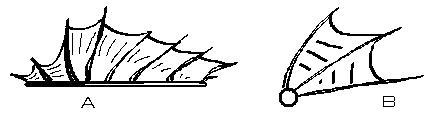
\includegraphics[width=\textwidth]{../images/styles/rlaan-fins.png}
}
    \caption{Rlaan fins with a higher number of ribs for large vessels.}
    \label{fig:rlaan-fins}
\end{center}
\end{figure}

\begin{figure} \begin{center}
	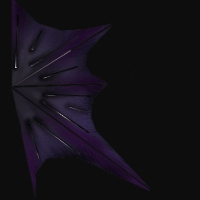
\includegraphics[width=0.4\textwidth]{../images/styles/rlaan-fins2.png}
    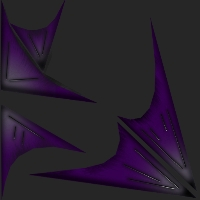
\includegraphics[width=0.4\textwidth]{../images/styles/rlaan-fins3.png}
    \caption{Samples of fin textures from in-game Rlaan ships.}
    \label{fig:rlaan-fins2}
\end{center} \end{figure}


3. Basic form is smooth and flowing, totally organic. Bilateral symmetry is a requirement 	for most of their ships. Bilateral symmetry is indicative to Rlaans of speed and agility (and 	also of 	spuriousness, contrasting their own lumbering radial symmetry - symbolic of 	precision and versatility - to the more common bilateral symmetry of other known species. 	Hence a bilaterally symmetrical vehicle is as attractive to an Rlaan as a sports car is to a 	human). Radially symmetrical ships do exist, though most are inexpensive civilian 	transports and utility ships.

4. Base Colors

5. Base Textures

	B. Listed below are the basic required features of all Rlaan installations:

	C. General Rlaan technological features (some features common in Rlaan art and architecture, devices, surface vehicles, etc.)


\subsubsection{Surface features of large vessels}

\subsubsection{Small things found on the hull of a large  vessel}
\begin{itemize}
\item Service/Maintenance hatches
\end{itemize}
{\it Somewhat larger things found on the hull of a large Aeran vessel:}
\begin{itemize}
\item Escape pod launcher ports
\end{itemize}
{\it Yet larger things ... :}
\begin{itemize}
\item Pinnace/lander launch bay (non-carrier vessels)
\end{itemize}

\subsection{Vessels Listing}

    1. Aidi(Rlaan Passenger Puddle Jumper) 
    2. Andi(Rlaan Sub-Orbital Cargo transport) 
    3. Chengdi(Rlaan Lander) 
    4. Chengzong(Rlaan Refuse and Salvage Scow) 
    5. Chongdi(Rlaan Cargo Shuttle) 
    6. Chudi(Rlaan Resupply Ship) 
    7. Daizong(Rlaan Methane Flight Tender) 
    8. Dezong(Rlaan Battleship) 
    9. Duanzong(Rlaan Orbital Sniper Ship) 
    10. Duzong(Rlaan Occupation Vessel) 
    11. Feidi(Rlaan Dropship) 
    12. Gaodi(Rlaan Forcible Compliance Planetary Drone Craft) 
    13. Gaozong(Rlaan Mobile Sensor Drone) 
    14. Gaozu(Rlaan Oxygen Flight Tender) 
    15. Gondi(Rlaan Colonization ship) 
    16. Gongti(Rlaan Oxygen client colonization ship) 
    17. Guangzong(Rlaan Repair/Maintenance craft) 
    18. Han(Rlaan Exploration Ship) 
    19. (Rlaan Constructed for non-Rlaan use) Janissary {Rlaan constructed Saahasayaay Heavy Fighter} 
    20. Shangdi(Rlaan Bulk Transport) 
    21. Shenzong(Rlaan Cargo mover) 
    22. Shizong(Rlaan Light Equalizer Ship) 
    23. Taizu(Rlaan Methane Breather Heavy Cargo Shuttle) 
    24. Wendi(Rlaan Prisoner Transport) 
    25. Wudi(Rlaan Ship Impound Transport) 
    26. Xianzong(Rlaan Mining Craft) 
    27. Xiaozong(Rlaan Patrol Corvette) 
    28. Xizong(Rlaan Oxygen Breather Heavy Cargo Shuttle) 
    29. Xuande(Rlaan Light Passenger Transport) 
    30. Xuanzong(Rlaan Gas Miner) 
    31. Yindi(Rlaan Equalizer Extermination Craft) 
    32. Zhaozong(Rlaan Heavy Equalizer Ship) 
    33. Zhezong(Rlaan Large Passenger Liner) 

\subsection{Stations Listing}

Note: For modelers wondering about the list of the Rlaan stations, there are none. Stations are not named, in the way ships are. But if you insist... ;) here's a list of the needed Rlaan installations. Don't worry, alien stations do not need to be necessarily obvious as to their functions, so if your station model looks Rlaan, it would certainly fit comfortably into any of the blank station spots. Please read guides above though for the specifics of some stations.

    1 Rlaan Medical
    2 Rlaan Factory
    3 Rlaan Research
    4 Rlaan Relay
    5 Rlaan-Briin Medical Procedure Station
    6 Rlaan-Briin Bio-mod Research
    7 Rlaan Prison Station
    8 Rlaan Repair and Salvage Station
    9 Rlaan Civilian Shipyard
    10 Rlaan Mining Base
    11 Rlaan Refinery
    12 Rlaan Military Shipyard)
    13 Rlaan Jump Point Fortifications
    14 Rlaan Weapons Platform
    15 Rlaan Anti-matter Refinery
    16 Rlaan Civilian Population Defense Redoubt
    17 Rlaan Asteroid Fighter Base
    18 Rlaan Fighter Barracks
    19 Rlaan Star Fortress


% LocalWords:  Aerans Aeran Artstyle Aera Pinnace Acrotatus Agasicles Agesilaus
% LocalWords:  Agesipolis Agis Alcmenes Anaxander Wiki Anaxandridas Rlaan Areus
% LocalWords:  Anaxidamus Ariston Charillus Cleombrotus Cleomenes Demaratus Uln
% LocalWords:  Theopompus Dorissus Echestratus Eurycratides Eurypon Leons Bzbr
% LocalWords:  Nicander Pausanias Pleistarchus UnAeranned Pleistoanax Andolian
% LocalWords:  Spaceborn's MacGyver Polydectes Polydorus EVAs Procles Prytanis
% LocalWords:  Soos Teleclus terraforming Aenethforming Zeuxidamus homeworld
% LocalWords:  coreward chemoreception Klk'k Aeneth ecologies Shmrn

\section{Portfolio: The Rlaan-Briin}
Ships overview for all groups (Work In Progress): \href{http://vegastrike.sourceforge.net/wiki/Artstyle\_guide:Overview\_Guide}{Ship Overview} \\
Art-style Guide (Work In Progress): \href{http://vegastrike.sourceforge.net/wiki/Artstyle\_guide:Rlaan-Briin}{Artstyle Guide} \\
Species overview: \href{http://vegastrike.sourceforge.net/wiki/Species:Rlaan}{Species:Rlaan} \\

\subsection{Origin}
\begin{itemize}
\item Gravity: 

\item Atmosphere: 

\item Primary liquid bodies: 

\item Average temperature of homeworld (pre-industrialization):

\item Sun: 

\item Primary challenges (pre-industrialization): 
\end{itemize}

%ORIGIN COMMENTS GO HERE

\subsubsection{Habitat}

\subsection{Physical}
\begin{itemize}
\item Dimensions: 

\item Mass: 

\item Skeletal system: 

\item Major divisions: 

\item Senses: 

\item Visual acuity: 

\item Chemosense: 

\item Locomotion: 

\item Manipulators: 

\item Textural appearance: 
\end{itemize}

%PHYSICAL COMMENTS GO HERE

\subsection{Mental}


\subsection{Technological}
\begin{itemize}
\item Tech: 


\item Weapons:

\item Tactics:
\begin{itemize}
\item    Small groups: 
\item    Large groups/Fleets: 
\end{itemize}


\item Installations:


\end{itemize}

\subsection{Culture}

\subsubsection{Factions and Organizational Groups}
Listed below are noteworthy Aeran sub-factions and organizational groups: 
\begin{itemize}
\item FACTIONS GO HERE
\end{itemize}

\subsubsection{Religion}

\subsubsection{Cultural Aesthetics}

\subsection{Writing, numbers, and insignia}

\subsection{Faction: PRIMARY FACTION}
%Faction data 
%Aera 
%Species 	Aera 
%Homeworld (Origin) 	Aeneth 
%Capital 	Aeneth 


\subsubsection{A Brief History of the PRIMARY FACTION}


\subsubsection{Development}

\subsubsection{Culture}

\subsubsection{Organization}

\subsection{Faction: OTHER FACTIONS}

%Faction data 
%Merchant Marines 
%Species 	Aera 
%Homeworld (Origin) 	Aeneth 
%Capital 	Aeneth 


\subsection{Vessels}

\subsubsection{Style Overview}
\begin{itemize}

\item Primary distinguishing color ranges: 

\item Common accent colors:

\item Primary lighting color:

\item Frequently visible: 

\item Rarely visible:

\item Seen inside, but not out: 

\item Moving parts(non-turret): 

\item Capital vs. light craft: 

\end{itemize}

\subsubsection{Surface features of large vessels}

\subsubsection{Small things found on the hull of a large  vessel}
\begin{itemize}
\item Service/Maintenance hatches
\end{itemize}
{\it Somewhat larger things found on the hull of a large Aeran vessel:}
\begin{itemize}
\item Escape pod launcher ports
\end{itemize}
{\it Yet larger things ... :}
\begin{itemize}
\item Pinnace/lander launch bay (non-carrier vessels)
\end{itemize}

\subsubsection{Listing of vessels}

\begin{itemize}
\item \href{http://vegastrike.sourceforge.net/wiki/Vessel:FOO}{FOO:} 

Existing concept art is not particularly canonical. Please redesign.

\end{itemize}

% LocalWords:  Aerans Aeran Artstyle Aera Pinnace Acrotatus Agasicles Agesilaus
% LocalWords:  Agesipolis Agis Alcmenes Anaxander Wiki Anaxandridas Rlaan Areus
% LocalWords:  Anaxidamus Ariston Charillus Cleombrotus Cleomenes Demaratus Uln
% LocalWords:  Theopompus Dorissus Echestratus Eurycratides Eurypon Leons Bzbr
% LocalWords:  Nicander Pausanias Pleistarchus UnAeranned Pleistoanax Andolian
% LocalWords:  Spaceborn's MacGyver Polydectes Polydorus EVAs Procles Prytanis
% LocalWords:  Soos Teleclus terraforming Aenethforming Zeuxidamus homeworld
% LocalWords:  coreward chemoreception Klk'k Aeneth ecologies Shmrn

\section{Portfolio: The Saahasayaay}
Ships overview for all groups (Work In Progress): \href{http://vegastrike.sourceforge.net/wiki/Artstyle\_guide:Overview\_Guide}{Ship Overview} \\
Art-style Guide (Work In Progress): \href{http://vegastrike.sourceforge.net/wiki/Artstyle\_guide:Saahasayaay}{Artstyle Guide} \\
Species overview: \href{http://vegastrike.sourceforge.net/wiki/Species:Saahasayaay}{Species:Saahasayaay} \\

\subsection{Origin}
\begin{itemize}
\item Gravity: 

\item Atmosphere: 

\item Primary liquid bodies: 

\item Average temperature of homeworld (pre-industrialization):

\item Sun: 

\item Primary challenges (pre-industrialization): 
\end{itemize}

%ORIGIN COMMENTS GO HERE

\subsubsection{Habitat}

\subsection{Physical}
\begin{itemize}
\item Dimensions: 

\item Mass: 

\item Skeletal system: 

\item Major divisions: 

\item Senses: 

\item Visual acuity: 

\item Chemosense: 

\item Locomotion: 

\item Manipulators: 

\item Textural appearance: 
\end{itemize}

%PHYSICAL COMMENTS GO HERE

\subsection{Mental}


\subsection{Technological}
\begin{itemize}
\item Tech: 


\item Weapons:

\item Tactics:
\begin{itemize}
\item    Small groups: 
\item    Large groups/Fleets: 
\end{itemize}


\item Installations:


\end{itemize}

\subsection{Culture}

\subsubsection{Factions and Organizational Groups}
Listed below are noteworthy Aeran sub-factions and organizational groups: 
\begin{itemize}
\item FACTIONS GO HERE
\end{itemize}

\subsubsection{Religion}

\subsubsection{Cultural Aesthetics}

\subsection{Writing, numbers, and insignia}

\subsection{Faction: PRIMARY FACTION}
%Faction data 
%Aera 
%Species 	Aera 
%Homeworld (Origin) 	Aeneth 
%Capital 	Aeneth 


\subsubsection{A Brief History of the PRIMARY FACTION}


\subsubsection{Development}

\subsubsection{Culture}

\subsubsection{Organization}

\subsection{Faction: OTHER FACTIONS}

%Faction data 
%Merchant Marines 
%Species 	Aera 
%Homeworld (Origin) 	Aeneth 
%Capital 	Aeneth 


\subsection{Vessels}

\subsubsection{Style Overview}
\begin{itemize}

\item Primary distinguishing color ranges: 

\item Common accent colors:

\item Primary lighting color:

\item Frequently visible: 

\item Rarely visible:

\item Seen inside, but not out: 

\item Moving parts(non-turret): 

\item Capital vs. light craft: 

\end{itemize}

\subsubsection{Surface features of large vessels}

\subsubsection{Small things found on the hull of a large  vessel}
\begin{itemize}
\item Service/Maintenance hatches
\end{itemize}
{\it Somewhat larger things found on the hull of a large Aeran vessel:}
\begin{itemize}
\item Escape pod launcher ports
\end{itemize}
{\it Yet larger things ... :}
\begin{itemize}
\item Pinnace/lander launch bay (non-carrier vessels)
\end{itemize}

\subsubsection{Listing of vessels}

\begin{itemize}
\item \href{http://vegastrike.sourceforge.net/wiki/Vessel:FOO}{FOO:} 

Existing concept art is not particularly canonical. Please redesign.

\end{itemize}

% LocalWords:  Aerans Aeran Artstyle Aera Pinnace Acrotatus Agasicles Agesilaus
% LocalWords:  Agesipolis Agis Alcmenes Anaxander Wiki Anaxandridas Rlaan Areus
% LocalWords:  Anaxidamus Ariston Charillus Cleombrotus Cleomenes Demaratus Uln
% LocalWords:  Theopompus Dorissus Echestratus Eurycratides Eurypon Leons Bzbr
% LocalWords:  Nicander Pausanias Pleistarchus UnAeranned Pleistoanax Andolian
% LocalWords:  Spaceborn's MacGyver Polydectes Polydorus EVAs Procles Prytanis
% LocalWords:  Soos Teleclus terraforming Aenethforming Zeuxidamus homeworld
% LocalWords:  coreward chemoreception Klk'k Aeneth ecologies Shmrn

\section{Portfolio: The Shapers}
Ships overview for all groups (Work In Progress): \href{http://vegastrike.sourceforge.net/wiki/Artstyle\_guide:Overview\_Guide}{Ship Overview} \\
Art-style Guide (Work In Progress): \href{http://vegastrike.sourceforge.net/wiki/Artstyle\_guide:Shaper}{Artstyle Guide} \\
Species overview: \href{http://vegastrike.sourceforge.net/wiki/Species:Humanity}{Species:Humanity} \\

\subsection{Origin}
\begin{itemize}
\item Sector: 
\item System: 
\item Origin Planet:  
\item Gravity: 

\item Atmosphere: 

\item Primary liquid bodies: 

\item Average temperature of homeworld (pre-industrialization):

\item Sun: 

\item Primary challenges (pre-industrialization): 
\end{itemize}

%ORIGIN COMMENTS GO HERE

\subsubsection{Habitat}

\subsection{Physical}
\begin{itemize}
\item Dimensions: 

\item Mass: 

\item Skeletal system: 

\item Major divisions: 

\item Senses: 

\item Visual acuity: 

\item Chemosense: 

\item Locomotion: 

\item Manipulators: 

\item Textural appearance: 
\end{itemize}

%PHYSICAL COMMENTS GO HERE

\subsection{Mental}


\subsection{Technological}
\begin{itemize}
\item Tech: 


\item Weapons:

\item Tactics:
\begin{itemize}
\item    Small groups: 
\item    Large groups/Fleets: 
\end{itemize}


\item Installations:


\end{itemize}

\subsection{Culture}

\subsubsection{Factions and Organizational Groups}
Listed below are noteworthy Aeran sub-factions and organizational groups: 
\begin{itemize}
\item FACTIONS GO HERE
\end{itemize}

\subsubsection{Religion}

\subsubsection{Cultural Aesthetics}

\subsection{Writing, numbers, and insignia}

\subsection{Faction: PRIMARY FACTION}
%Faction data 
%Aera 
%Species 	Aera 
%Homeworld (Origin) 	Aeneth 
%Capital 	Aeneth 


\subsubsection{A Brief History of the PRIMARY FACTION}


\subsubsection{Development}

\subsubsection{Culture}

\subsubsection{Organization}

\subsection{Faction: OTHER FACTIONS}

%Faction data 
%Merchant Marines 
%Species 	Aera 
%Homeworld (Origin) 	Aeneth 
%Capital 	Aeneth 


\subsection{Vessels}

\subsubsection{Style Overview}
\begin{itemize}

\item Primary distinguishing color ranges: 

\item Common accent colors:

\item Primary lighting color:

\item Frequently visible: 

\item Rarely visible:

\item Seen inside, but not out: 

\item Moving parts(non-turret): 

\item Capital vs. light craft: 

\end{itemize}

\subsubsection{Surface features of large vessels}

\subsubsection{Small things found on the hull of a large  vessel}
\begin{itemize}
\item Service/Maintenance hatches
\end{itemize}
{\it Somewhat larger things found on the hull of a large Aeran vessel:}
\begin{itemize}
\item Escape pod launcher ports
\end{itemize}
{\it Yet larger things ... :}
\begin{itemize}
\item Pinnace/lander launch bay (non-carrier vessels)
\end{itemize}

\subsubsection{Listing of vessels}

\begin{itemize}
\item \href{http://vegastrike.sourceforge.net/wiki/Vessel:FOO}{FOO:} 

Existing concept art is not particularly canonical. Please redesign.

\end{itemize}

% LocalWords:  Aerans Aeran Artstyle Aera Pinnace Acrotatus Agasicles Agesilaus
% LocalWords:  Agesipolis Agis Alcmenes Anaxander Wiki Anaxandridas Rlaan Areus
% LocalWords:  Anaxidamus Ariston Charillus Cleombrotus Cleomenes Demaratus Uln
% LocalWords:  Theopompus Dorissus Echestratus Eurycratides Eurypon Leons Bzbr
% LocalWords:  Nicander Pausanias Pleistarchus UnAeranned Pleistoanax Andolian
% LocalWords:  Spaceborn's MacGyver Polydectes Polydorus EVAs Procles Prytanis
% LocalWords:  Soos Teleclus terraforming Aenethforming Zeuxidamus homeworld
% LocalWords:  coreward chemoreception Klk'k Aeneth ecologies Shmrn

\section{Portfolio: The Shmrn}
Ships overview for all groups (Work In Progress): \href{http://vegastrike.sourceforge.net/wiki/Artstyle\_guide:Overview\_Guide}{Ship Overview} \\
Art-style Guide (Work In Progress): \href{http://vegastrike.sourceforge.net/wiki/Artstyle\_guide:Shmrn}{Artstyle Guide} \\
Species overview: \href{http://vegastrike.sourceforge.net/wiki/Species:Shmrn}{Species:Shmrn} \\

\subsection{Origin}
\begin{itemize}
\item Sector: 
\item System: 
\item Origin Planet:  
\item Gravity: 

\item Atmosphere: 

\item Primary liquid bodies: 

\item Average temperature of homeworld (pre-industrialization):

\item Sun: 

\item Primary challenges (pre-industrialization): 
\end{itemize}

%ORIGIN COMMENTS GO HERE

\subsubsection{Habitat}

\subsection{Physical}
\begin{itemize}
\item Dimensions: 

\item Mass: 

\item Skeletal system: 

\item Major divisions: 

\item Senses: 

\item Visual acuity: 

\item Chemosense: 

\item Locomotion: 

\item Manipulators: 

\item Textural appearance: 
\end{itemize}

%PHYSICAL COMMENTS GO HERE

\subsection{Mental}


\subsection{Technological}
\begin{itemize}
\item Tech: 


\item Weapons:

\item Tactics:
\begin{itemize}
\item    Small groups: 
\item    Large groups/Fleets: 
\end{itemize}


\item Installations:


\end{itemize}

\subsection{Culture}

\subsubsection{Factions and Organizational Groups}
Listed below are noteworthy Aeran sub-factions and organizational groups: 
\begin{itemize}
\item FACTIONS GO HERE
\end{itemize}

\subsubsection{Religion}

\subsubsection{Cultural Aesthetics}

\subsection{Writing, numbers, and insignia}

\subsection{Faction: PRIMARY FACTION}
%Faction data 
%Aera 
%Species 	Aera 
%Homeworld (Origin) 	Aeneth 
%Capital 	Aeneth 


\subsubsection{A Brief History of the PRIMARY FACTION}


\subsubsection{Development}

\subsubsection{Culture}

\subsubsection{Organization}

\subsection{Faction: OTHER FACTIONS}

%Faction data 
%Merchant Marines 
%Species 	Aera 
%Homeworld (Origin) 	Aeneth 
%Capital 	Aeneth 


\subsection{Vessels}

\subsubsection{Style Overview}
\begin{itemize}

\item Primary distinguishing color ranges: 

\item Common accent colors:

\item Primary lighting color:

\item Frequently visible: 

\item Rarely visible:

\item Seen inside, but not out: 

\item Moving parts(non-turret): 

\item Capital vs. light craft: 

\end{itemize}

\subsubsection{Surface features of large vessels}

\subsubsection{Small things found on the hull of a large  vessel}
\begin{itemize}
\item Service/Maintenance hatches
\end{itemize}
{\it Somewhat larger things found on the hull of a large Aeran vessel:}
\begin{itemize}
\item Escape pod launcher ports
\end{itemize}
{\it Yet larger things ... :}
\begin{itemize}
\item Pinnace/lander launch bay (non-carrier vessels)
\end{itemize}

\subsubsection{Listing of vessels}

\begin{itemize}
\item \href{http://vegastrike.sourceforge.net/wiki/Vessel:FOO}{FOO:} 

Existing concept art is not particularly canonical. Please redesign.

\end{itemize}

% LocalWords:  Aerans Aeran Artstyle Aera Pinnace Acrotatus Agasicles Agesilaus
% LocalWords:  Agesipolis Agis Alcmenes Anaxander Wiki Anaxandridas Rlaan Areus
% LocalWords:  Anaxidamus Ariston Charillus Cleombrotus Cleomenes Demaratus Uln
% LocalWords:  Theopompus Dorissus Echestratus Eurycratides Eurypon Leons Bzbr
% LocalWords:  Nicander Pausanias Pleistarchus UnAeranned Pleistoanax Andolian
% LocalWords:  Spaceborn's MacGyver Polydectes Polydorus EVAs Procles Prytanis
% LocalWords:  Soos Teleclus terraforming Aenethforming Zeuxidamus homeworld
% LocalWords:  coreward chemoreception Klk'k Aeneth ecologies Shmrn

\section{Portfolio: The Uln}
Ships overview for all groups (Work In Progress): \href{http://vegastrike.sourceforge.net/wiki/Artstyle\_guide:Overview\_Guide}{Ship Overview} \\
Art-style Guide (Work In Progress): \href{http://vegastrike.sourceforge.net/wiki/Artstyle\_guide:Uln}{Artstyle Guide} \\
Species overview: \href{http://vegastrike.sourceforge.net/wiki/Species:Uln}{Species:Uln} \\

\subsection{Origin}
\begin{itemize}
\item Sector: 
\item System: 
\item Origin Planet:  
\item Gravity: 

\item Atmosphere: 

\item Primary liquid bodies: 

\item Average temperature of homeworld (pre-industrialization):

\item Sun: 

\item Primary challenges (pre-industrialization): 
\end{itemize}

%ORIGIN COMMENTS GO HERE

\subsubsection{Habitat}

\subsection{Physical}
\begin{itemize}
\item Dimensions: 

\item Mass: 

\item Skeletal system: 

\item Major divisions: 

\item Senses: 

\item Visual acuity: 

\item Chemosense: 

\item Locomotion: 

\item Manipulators: 

\item Textural appearance: 
\end{itemize}

%PHYSICAL COMMENTS GO HERE

\subsection{Mental}


\subsection{Technological}
\begin{itemize}
\item Tech: 


\item Weapons:

\item Tactics:
\begin{itemize}
\item    Small groups: 
\item    Large groups/Fleets: 
\end{itemize}


\item Installations:


\end{itemize}

\subsection{Culture}

\subsubsection{Factions and Organizational Groups}
Listed below are noteworthy Aeran sub-factions and organizational groups: 
\begin{itemize}
\item FACTIONS GO HERE
\end{itemize}

\subsubsection{Religion}

\subsubsection{Cultural Aesthetics}

\subsection{Writing, numbers, and insignia}

\subsection{Faction: PRIMARY FACTION}
%Faction data 
%Aera 
%Species 	Aera 
%Homeworld (Origin) 	Aeneth 
%Capital 	Aeneth 


\subsubsection{A Brief History of the PRIMARY FACTION}


\subsubsection{Development}

\subsubsection{Culture}

\subsubsection{Organization}

\subsection{Faction: OTHER FACTIONS}

%Faction data 
%Merchant Marines 
%Species 	Aera 
%Homeworld (Origin) 	Aeneth 
%Capital 	Aeneth 


\subsection{Vessels}

\subsubsection{Style Overview}
\begin{itemize}

\item Primary distinguishing color ranges: 

\item Common accent colors:

\item Primary lighting color:

\item Frequently visible: 

\item Rarely visible:

\item Seen inside, but not out: 

\item Moving parts(non-turret): 

\item Capital vs. light craft: 

\end{itemize}

\subsubsection{Surface features of large vessels}

\subsubsection{Small things found on the hull of a large  vessel}
\begin{itemize}
\item Service/Maintenance hatches
\end{itemize}
{\it Somewhat larger things found on the hull of a large Aeran vessel:}
\begin{itemize}
\item Escape pod launcher ports
\end{itemize}
{\it Yet larger things ... :}
\begin{itemize}
\item Pinnace/lander launch bay (non-carrier vessels)
\end{itemize}

\subsubsection{Listing of vessels}

\begin{itemize}
\item \href{http://vegastrike.sourceforge.net/wiki/Vessel:FOO}{FOO:} 

Existing concept art is not particularly canonical. Please redesign.

\end{itemize}

% LocalWords:  Aerans Aeran Artstyle Aera Pinnace Acrotatus Agasicles Agesilaus
% LocalWords:  Agesipolis Agis Alcmenes Anaxander Wiki Anaxandridas Rlaan Areus
% LocalWords:  Anaxidamus Ariston Charillus Cleombrotus Cleomenes Demaratus Uln
% LocalWords:  Theopompus Dorissus Echestratus Eurycratides Eurypon Leons Bzbr
% LocalWords:  Nicander Pausanias Pleistarchus UnAeranned Pleistoanax Andolian
% LocalWords:  Spaceborn's MacGyver Polydectes Polydorus EVAs Procles Prytanis
% LocalWords:  Soos Teleclus terraforming Aenethforming Zeuxidamus homeworld
% LocalWords:  coreward chemoreception Klk'k Aeneth ecologies Shmrn

\section{Portfolio: The Unadorned}
Ships overview for all groups (Work In Progress): \href{http://vegastrike.sourceforge.net/wiki/Artstyle\_guide:Overview\_Guide}{Ship Overview} \\
Art-style Guide (Work In Progress): \href{http://vegastrike.sourceforge.net/wiki/Artstyle\_guide:Unadorned}{Artstyle Guide} \\
Species overview: \href{http://vegastrike.sourceforge.net/wiki/Species:Humanity}{Species:Humanity} \\

\subsection{Origin}
\begin{itemize}
\item Sector: 
\item System: 
\item Origin Planet:  
\item Gravity: 

\item Atmosphere: 

\item Primary liquid bodies: 

\item Average temperature of homeworld (pre-industrialization):

\item Sun: 

\item Primary challenges (pre-industrialization): 
\end{itemize}

%ORIGIN COMMENTS GO HERE

\subsubsection{Habitat}

\subsection{Physical}
\begin{itemize}
\item Dimensions: 

\item Mass: 

\item Skeletal system: 

\item Major divisions: 

\item Senses: 

\item Visual acuity: 

\item Chemosense: 

\item Locomotion: 

\item Manipulators: 

\item Textural appearance: 
\end{itemize}

%PHYSICAL COMMENTS GO HERE

\subsection{Mental}


\subsection{Technological}
\begin{itemize}
\item Tech: 


\item Weapons:

\item Tactics:
\begin{itemize}
\item    Small groups: 
\item    Large groups/Fleets: 
\end{itemize}


\item Installations:


\end{itemize}

\subsection{Culture}

\subsubsection{Factions and Organizational Groups}
Listed below are noteworthy Aeran sub-factions and organizational groups: 
\begin{itemize}
\item FACTIONS GO HERE
\end{itemize}

\subsubsection{Religion}

\subsubsection{Cultural Aesthetics}

\subsection{Writing, numbers, and insignia}

\subsection{Faction: PRIMARY FACTION}
%Faction data 
%Aera 
%Species 	Aera 
%Homeworld (Origin) 	Aeneth 
%Capital 	Aeneth 


\subsubsection{A Brief History of the PRIMARY FACTION}


\subsubsection{Development}

\subsubsection{Culture}

\subsubsection{Organization}

\subsection{Faction: OTHER FACTIONS}

%Faction data 
%Merchant Marines 
%Species 	Aera 
%Homeworld (Origin) 	Aeneth 
%Capital 	Aeneth 


\subsection{Vessels}

\subsubsection{Style Overview}
\begin{itemize}

\item Primary distinguishing color ranges: 

\item Common accent colors:

\item Primary lighting color:

\item Frequently visible: 

\item Rarely visible:

\item Seen inside, but not out: 

\item Moving parts(non-turret): 

\item Capital vs. light craft: 

\end{itemize}

\subsubsection{Surface features of large vessels}

\subsubsection{Small things found on the hull of a large  vessel}
\begin{itemize}
\item Service/Maintenance hatches
\end{itemize}
{\it Somewhat larger things found on the hull of a large Aeran vessel:}
\begin{itemize}
\item Escape pod launcher ports
\end{itemize}
{\it Yet larger things ... :}
\begin{itemize}
\item Pinnace/lander launch bay (non-carrier vessels)
\end{itemize}

\subsubsection{Listing of vessels}

\begin{itemize}
\item \href{http://vegastrike.sourceforge.net/wiki/Vessel:FOO}{FOO:} 

Existing concept art is not particularly canonical. Please redesign.

\end{itemize}

% LocalWords:  Aerans Aeran Artstyle Aera Pinnace Acrotatus Agasicles Agesilaus
% LocalWords:  Agesipolis Agis Alcmenes Anaxander Wiki Anaxandridas Rlaan Areus
% LocalWords:  Anaxidamus Ariston Charillus Cleombrotus Cleomenes Demaratus Uln
% LocalWords:  Theopompus Dorissus Echestratus Eurycratides Eurypon Leons Bzbr
% LocalWords:  Nicander Pausanias Pleistarchus UnAeranned Pleistoanax Andolian
% LocalWords:  Spaceborn's MacGyver Polydectes Polydorus EVAs Procles Prytanis
% LocalWords:  Soos Teleclus terraforming Aenethforming Zeuxidamus homeworld
% LocalWords:  coreward chemoreception Klk'k Aeneth ecologies Shmrn

%input{profile_}

% LocalWords:  UtCS
